\chapter{Spectrum Allocation in TV White Space complying with ECC Rulings}
% Distributed Channel and Power Allocation in IEEE 802.22 Networks
\begin{quote}
{\textbf{Abstract}\\
\small In this chapter, we will see the application of congestion game in solving the channel allocation problem in the context of TV white space.
The channel allocation problem we will address is a general problem, as the transmission power is not identical for every transmitter and on each channel, actually, the transmission power could be unique for each transmitter-channel combination.
With the suitable utility function designed for transmitters, the behaviours of the transmitters can be described by a congestion game.
The algorithm of channel allocation is derived from the dynamics of the transmitter in the game, which reaches Nash equilibrium quickly.

Furthermore, we provide a complete solution to fully exploit TV white space complying with IEEE 802.22 standard.
We propose a centralized methods to regulate the upper bound of transmission power, so that to strictly protect the primary users.
%Proposed scheme also considers the necessity of distributable execution which decides the working channel and transmission power.
The the distributed channel allocation and power control are conducted sequentially.
%As to the channel allocation problem, we innovatively formulate this problem in to a canonical congestion game, and design efficient distributed channel selection strategy with the assistance of the centralized database.
%The successful practice of congestion game in this problem is enlightening for the application of congestion game in other problems where asymmetric interaction exists.
}
\end{quote}

\section{Introduction}



%%%%%%%%%%%%%%%%%%%%%%%%%%%%%%%%%%%%%%%%%%%%%%%%%%%%%

Secondary users working with TV white space is promising to cope with the scarcity of spectrum resources~\cite{FCC_2010_sedond_memorandumm}. 
Firstly, more unused TV white frequencies become vacant than ever with the ongoing transition from analog to digital broadcasts. Secondly, the frequencies of TV bands enable broadband access over larger geographic ranges compared to higher frequency bands. Nevertheless, services on TV receivers need to be protected with so called interference margin~\footnote{interference margin is the maximal interference caused by secondary users, which doesn't violate TV service.}~\cite{multipleIntf_pimrc11} which should not be exceeded by the accumulated interference caused by all secondary users working on the the channel.

\gls{FCC} and \gls{ECC} have announced rules on the transmission power of secondary users working in TV white space in US and Europe respectively~\cite{FCC_2010_sedond_memorandumm, ecc159}. 
FCC requires a minimum distance between secondary user and TV service area, besides, the transmission power for fixed secondary users is set as $4$ \textup{W}, which is a conservative setting. %If the interference margin of the TV receivers can be fully utilized, the requirement on secondary users' transmission power can be relaxed to some extent. 
FCC believes with these prudent measures, the interference margin can not be exceeded by interference from secondary users.
But it may not be the case when there are multiple secondary equipments transmitting at the same time, which is pointed in~\cite{Jaentti11}.
ECC requires the secondary users to adapt their maximum transmission power according to the distance away from the TV receivers.
%In this manner, secondary systems have to determine their maximum transmission power.

\begin{figure}[h!]
  \centering
  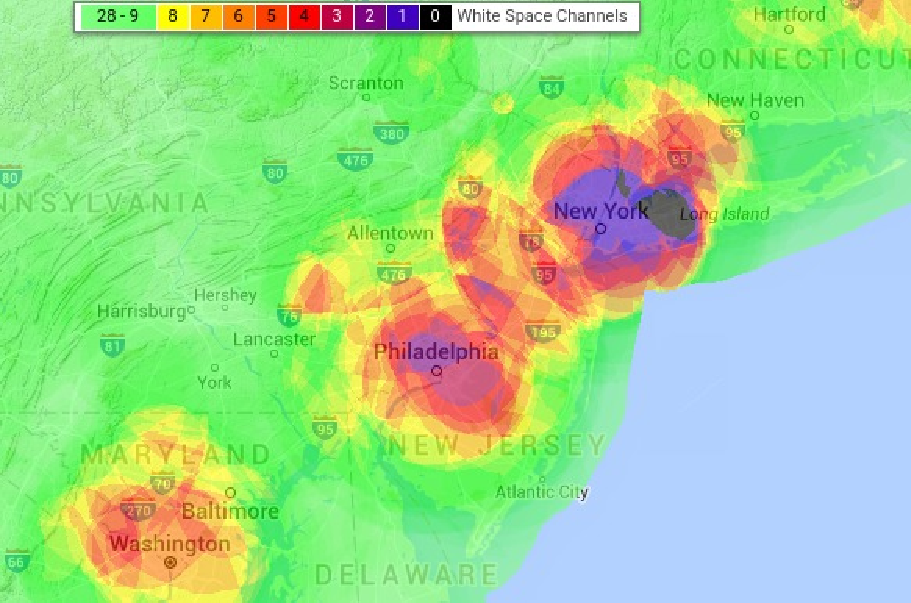
\includegraphics[width=0.9\linewidth]{TWWS_availability_east.pdf}
  \caption{Variability of available channels in a densely populated area. This figure is obtained from \cite{googleDatabase}}
\label{variability_avai_channel}
\end{figure}


FCC issued a memorandum~\cite{FCC_2010_sedond_memorandumm,FCCdatabasae} in 2010, which removes the mandatory rigid sensing requirements, and prompts the usage of geolocations\footnote{Geolocation means both geographic location and terrain.} of secondary users.
FCC regulates a centralized database, which registers all the secondary users within one certain area.
Secondary users can access the database, and can only use the channels assigned by the database.
% thus greatly facilitates the use of the spectrum with geolocation based channel allocation.
Work~\cite{SenseLess2011} follows this rule to obviate spectrum sensing and only relies on the database of TV incumbents to determine the white space availability for secondary users. 
The authors of~\cite{SenseLess2011} demonstrate the feasibility of predicting the available TV spectrum accurately using sophisticated propagation models (Longley-Rice) and geolocations of secondary users. 
A central database contains the geolocations of all TV stations, then the database calculates the received signal strength index (\gls{RSSI}) levels of TV \gls{UHF} signals on all secondary users and accordingly determines the available TV spectrum for them. 
If RSSI of a channel is below a certain threshold, TV service is regarded not to exist, and the channel is seen available there.
The calculated results on channel availability is very close to the measurement results.
The work of~\cite{SenseLess2011} gives big impetus to the usage of database mode.
%
%Through this work, it can be seen that the RSSI level caused by secondary users on TV receivers can be calculated accurately in a centralized entity if secondary users' transmission power, geographic location and appropriate propagation model are provided. 
As in TV white space, the accurate RSSI can be obtained with geolocations and suitable propagation model, given geolocation and appropriate propagation model, secondary users' maximum transmission power can be determined by the central entity according to the interference margin (maximum RSSI level from secondary users) on the TV receivers. 
%Obviously, transmission power control of secondary users has a significant impact on the performance of these systems. 

%To guarantee the protection on TV systems from harmful interference, FCC and IEEE propose a central database to regulate the access of TV spectrum by the secondary users.
%The centralized database registers the location and terrain information for all secondary users in the network, and decides the available channel and maximal permitted transmission power for each secondary user. 

%, and meanwhile the aggregated interference generated by them should be kept below a certain threshold on the TV system.

In this chapter, we investigate the usage of TV spectrum in a wireless regional area network which complies with IEEE 802.22 network.
The secondary users are assumed to be cellular base stations and associated terminals, all of which work on TV white spectrum. 
The base station is referred as WBS.
%The corresponding secondary base stations are referred as white base stations (WBS). 
Some cellular networks, \ie GSM or LTE network, work on licensed spectrum and emphasis on providing satisfactory services to their end terminals by choosing proper transmission channel and power. 
As to cellular network working on TV white spectrum, they have to keep one eye on the primary users to make sure that TV service is not violated, which makes the problem of channel and power selection difficult.
With the existence of central database, it is natural to utilize it as a central controller to assign channel and power usage for secondary users, but the secondary users may belong to different commercial groups and they may not contend with the assigned resource.
%Besides, as the TV channels have different quality, \ie interference level, and permitted transmission power, it is difficult for the database to assign them to the 
Hence, the spectrum sharing of the secondary users in IEEE 802.22 network should be decided in distributed manner and each secondary user takes care of its own interest, \ie to maximize its preferred utility.

Given all the other WBSs' selection on channel and transmission power, a WBS is interested in choosing the channel which brings it the best performance, \ie the data rate of its end users.
A WBS prefers to choose the channel which experiences the minimum interference, and the transmission power allowed on that channel is higher, so as to obtain better SINR on its terminals and meanwhile maximize their coverage \cite{wuinfocom09, HoangPowerChannel2010}. 
Nevertheless, high transmission power causes significant co-channel interference to other secondary users operating on the same channel. 
Hence, a secondary cell has to balance its transmission power and the caused interference on other cells, meanwhile to choose working channel to decrease the experienced interference on its terminals. 
The goal of this chapter is to protect the primary users from harmful interferences, meanwhile to find a strategy for WBSs to choose channel and power level in order to acquire good SINR on end terminals.

The rest of the chapter is organized as follows. we elucidate the system model in Section II, afterwards related work and problem formulation is presented in Section III. In Section IV, we discuss how to utilize the white space sufficiently by setting the transmission powers based on a convex problem formulation. We analyze the spectrum allocation problem under game theoretical framework and propose an algorithm in Section V, thereafter performance evaluation is presented in Section VI. Finally, we conclude our work and point out directions of future research in Section VII.


\section{System Model and Problem Statement}
\label{SystemModel}
%According to the IEEE 802.22 standard, the primary systems considered in this chapter are digital TV (DTV) stations which use the TV spectrum legally. 
%TV stations provide service to passive TV receivers.
%The secondary users are IEEE 802.22 Wireless Regional Area Network base stations utilizing the TV spectrum with senseless mode~\cite{SenseLess2011}. 
%DTV's service should not be interfered by secondary systems. 

We consider an IEEE 802.22 compliant cellular network where the fixed white space devices work as base station and provide broadband access to their terminals.
The network is illustrated in Figure~\ref{sysmodel}.
We call the fixed white space devices which work as base stations as White space Base Stations (WBSs), they are located in one area which is surrounded by digital TV stations and receivers.
Several critical points are deployed in the vicinity of the digital TV receivers which are the most venerable to the interference caused by the white space devices.
WBSs work in underlay manner and coexist with the digital TV stations and receivers, the aggregate interference generated by WBSs should not exceed the threshold on each channel at each critical point.
%The aggregated interference on these critical points should below a certain threshold on all of the TVWS channels.
%
As to the WBSs, the out-of-band emission is regard as trivial, therefore, we only consider co-channel interference among the WBSs.
To simplify the analysis, we assume that each digital TV station as well as each WBS utilizes exactly one channel.\footnote{The assumption that one WBS only utilizes one channel is for convenience of analysis. In reality multiple channel usage (channel bonding) is requirement as one single TV channel's bandwidth is 6 MHz which is not adequate for a WBS to fulfill terminal demands. 
%We will relax this single channel usage assumption without hammering our scheme in the end of section \ref{sec_CA}.
}
%

As to the notations, the set of WBSs is denoted as $\mathcal{N}$ where $|\mathcal{N}|=N$. 
The TVWS spectrum bands are denoted as set $\mathbb{C}$.
We represent the usage of channel for WBS $i$ with a binary vector $X_i^{|\mathbb{C}|\times 1}=\{x_i^1,\cdots, x_i^k,\cdots, x_i^{|\mathbb{C}|}\}\in \{0,1\}^{|\mathbb{C}|}$, where $k\in \mathbb{C}$ and binary variable $x_i^k$ denotes whether channel $k$ is used by user $i$. 
All the WBSs work with the channels approved by the WSDB, they operate with a channel from the approved ones after choosing it, thus we omit the time index in the channel usage.
As each node can only uses one channel, for $X_i$, there is $\sum_{k=1}^{|\mathbb{C}|}x_i^k=1$. 
The transmission power of WBS $i$ on channel $c$ is $P_i^c$.
$c(i)$ denotes the channel used by a WBS $i\in \mathcal{N}$. 

\begin{figure}[h!]
  \centering
  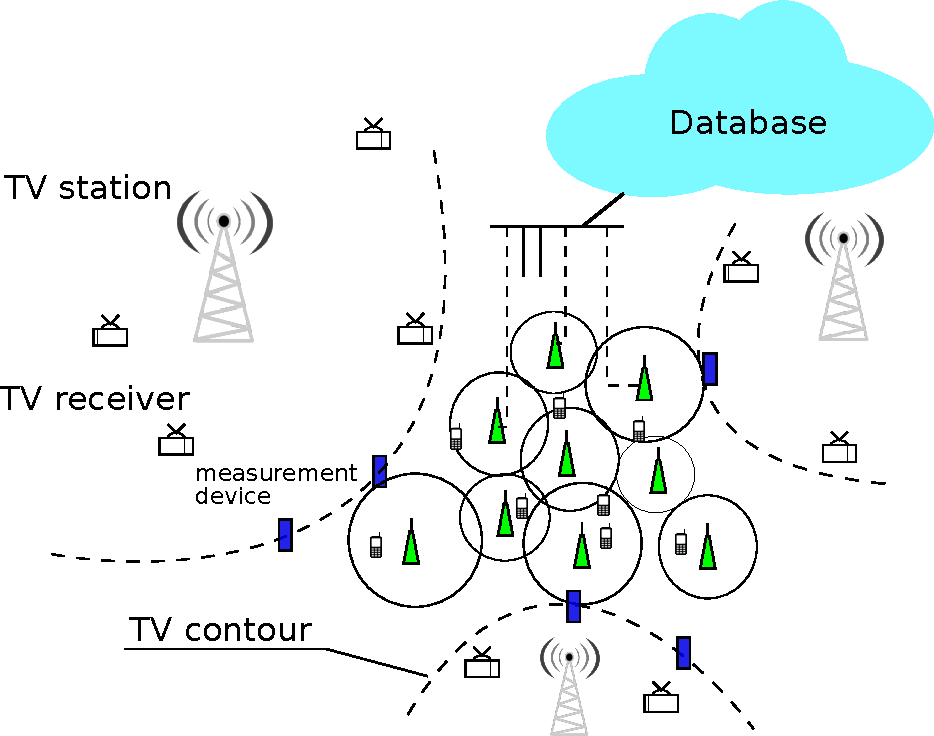
\includegraphics[width=0.9\linewidth]{systemmodel_working.pdf}
  \caption{System model: WBS cells and digital TV (DTV) systems}
\label{sysmodel}
\end{figure}
%In the rest of the chapter, we use WBS and secondary base station interchangeably. 
%There are interference measurement equipments deployed on the contours of TV service areas (as bold rectangles in Fig.~\ref{sysmodel}), which represent the worst located TV receivers in the TV service areas. 
%For these interference measurement devices, an interference threshold should not be violated by the noise generated by the secondary users.
%The deployment of the interference measurement devices is decided by the TV operators, which are usually along the contour of the area where TV receivers reside.
%Thus, the locations of interference measurement devices vary according to the concrete location, geographic terrain and possible deployment of secondary networks. 
%%For simplicity, we assume there is only one contour deployed for one TV area. % \todo{is contour 'clear' now?}.
%WBSs are deemed to be static.
%We assume the secondary base stations are not under the same operators, thus there is no scheduling mechanism available among WBSs.


For a terminal $m$ which is associated to WBS $i$, the attenuation between WBS $i$ and $m$ is denoted as $h_{im}$.
For the attenuation, we only take path loss and shadowing into account in the following.
The path loss is dependent on the distance between the corresponding equipment, e.g. $h_{im}=K \cdot d_{im}^{-\alpha}$, where $\alpha$ is the path loss exponent, $d_{im}$ is the distance between $i$ and $m$, while $K$ is a constant which models the reference loss over a single unit of distance.
Shadowing without fading is considered in our model.
$z_{im}$ models the zero-mean log-normally distributed shadow fading between $i$ and $m$, with the standard deviation $\sigma_{\text{SH}}$.
$N_0$ denotes the thermal noise power.
%
%The sum of all disturbing radio frequency effects (including interference) on terminal $m$ (we assume the working channel is $c$) is as following,
%\begin{equation}
%\label{interference}
%\begin{aligned}
%f_m^c=\sum_{\bar{i}} (P_{j}^c \cdot h_{jm} \cdot z_{jm}) +  N_0, \quad \quad j\in \mathcal{N}\setminus i, c(j) = c
%\end{aligned}
%\end{equation}
%where $P_{j}^c$ denotes the transmission power of interfering WBS $j$.
%Note that $z$ is dependent on the individual transmitter/receiver pair, but we omit the subscripts for simplicity. 
The SINR at end terminal $m$ is,
\begin{equation}
\label{SINR}
\begin{aligned}
\gamma_{m}  & = \frac{P_{i}^c \cdot h_{im}\cdot z_{im}} {f_m^c} & = \frac{P_{i}^c \cdot h_{im}\cdot z_{im}} {\sum (P_{j}^c \cdot h_{jm} \cdot z_{jm}) +  N_0}\\
					& &, \quad \quad j\in \mathcal{N}\setminus i, c(j) = c
\end{aligned}
\end{equation}
where $P_{j}^c$ denotes the transmission power of interfering WBS $j$.



%\subsection{Problem Statement}
In our model, we only assume the WBSs, which work with high transmission power, as the potential interfering unlicensed devices to the DTV service, meanwhile, WBSs are interested in providing broadband access to their associated terminals.
Our goal in this paper is to assign TVWS channel to each WBS so as to improve the signal to noise and interference ratio (SINR) of their associated end terminals, meanwhile complying with the ECC regulations.
The channels in $\mathbb{C}$ are assumed to be identical in terms of attenuation and shadowing on the same path.
%As to performance metric for the QoS provisioning, we choose the signal to noise and interference ratio (SINR) on the terminals.
A WBS's utility is a function of the SINR on all its end terminals, \ie the average SINR at all its terminals.


\subsection{Problem Formulation}
\label{problemProposed}
When we look for a metric for WBS, which represents the SINR on end users, it is not appropriate to choose only one terminal, as done in~\cite{spectrum_sharing_tvspace_2012}, or multiple fixed terminals to represent the all the terminals in the cell, because the locations of the chosen terminal could diverge greatly with respect to the other terminals.
Thus, we propose a metric \textit{QuasiSINR} to represent WBS's performance in terms of SINR on its end terminals, which is independent on the actual locations of end terminals.

Our goal is to minimize the sum of inverted SINR the WBSs $\sum_{i\in \mathcal{N}}\frac{1}{\gamma_{i}}$ .
We minimize the sum of inverted quasiSINR instead of maximizing the sum of quasiSINR in order to ensure the fairness among WBSs,  .
With an auxiliary circle centered at the discussed WBS, which is shown as dashed circle in Figure~\ref{quasiSINRfigure}, QuasiSINR is the ratio between the power of signal of interest on the circle and the summation of the strongest power from the interfering WBSs on the auxiliary circle.


\begin{figure}[h!]
  \centering
  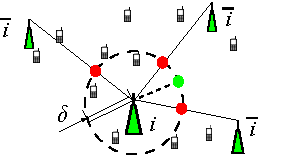
\includegraphics[width=0.6\linewidth]{quasiSINR2_2.pdf}
  \caption{Assuming the radius of the auxiliary circle is $\delta$ and all the WBSs work on the a channel, then QuasiSINR is a quotient where the divided is the WBS $i$'s power on the auxiliary circle (\ie the green pot), and the divisor is the summation of the interfering power on the red pots.}
\label{quasiSINRfigure}
\end{figure}

The quasiSINR of WBS $i$ is denoted as $\gamma_{i}$, 



\begin{equation}
\label{quasiSINR}
\begin{aligned}
 \gamma_{i} = &\frac{P_{i}^c \cdot h_{i\rightarrow \text{i's}\hspace{0.2em} \text{auxiliary circle}}\cdot z_{i\rightarrow \text{i's}\hspace{0.2em}\text{auxiliary circle}}} {\sum\limits_{\tiny\substack{j\neq i, j\in \mathcal{N}\\c(j)=c(i)}} (P_j^c \cdot h_{j\rightarrow \text{i's}\hspace{0.2em} \text{auxiliary circle}} \cdot z_{j\rightarrow \text{i's}\hspace{0.2em} \text{auxiliary circle}}) + N_0}\\
 = & \frac{P_{i}^c \cdot \delta^{-\alpha}\cdot z_{i\rightarrow \text{auxiliary circle}}} {\sum\limits_{\tiny\substack{j\neq i, j\in \mathcal{N}\\c(j)=c(i)}} (P_j^c \cdot (d_{ji}-\delta)^{-\alpha} \cdot z_{j\rightarrow \text{auxiliary circle}}) + N_0}
\end{aligned}
\end{equation}

In the following paper, when we talk about the channel and power allocation with respect to WBS, the notation $h_{ij}$ denotes the attenuation between WBS $i$ to the auxiliary circle of WBS $j$.
$h_{i}$ denotes the attenuation between WBS $i$ to its own auxiliary circle.
Then $\gamma_i$ becomes,
\begin{equation}
\label{quasiSINR_2}
\begin{aligned}
 \gamma_{i} = 
  \frac{P_{i}^c \cdot h_i\cdot z_i} {\sum\limits_{\tiny\substack{j\neq i, j\in \mathcal{N}\\c(j)=c(i)}} (P_j^c \cdot h_{ji} \cdot z_{ji}) + N_0}
\end{aligned}
\end{equation}
The abbreviations and notations used in this paper are found in Table~\ref{tab1}.
%
%With auxiliary circle, the decision made by WBSs is independent on the distribution of the end terminals.
The radius of the auxiliary circle $\delta$ can be adapted to foster better service to the terminals in certain area, \ie a larger radius $\delta$ will take care of the SINR on the terminals reside far away and vice visa.


\begin{table}[h]
\caption{Notations}
\label{tab1}
\centering
\begin{tabular}{l p{12cm}}
\toprule
Abbr. & Description \\
Symbol & \\
\midrule
TVWS & TV white spaces\\
WSDB & white space database\\
WBS & white space base stations\\
$\gamma$ & QuasiSINR\\
$f_{ji}^c$  & The co-channel interference caused by WBS $j$ on the auxiliary circle of WBS $i$, $c$ is the working channel for both\\
$f_i^c$ & The sum of interference caused on the auxiliary circle of WBS $i$ \\
$P_i^c$		& The maximal permitted Tx power of WBS $i$ on channel $c$ (ECC solution)\\
%$P_\mu, P_{\mathtt{op}}$		& The minimum and maximal permitted Tx power of WBS $i$ (FCC solution)\\
$h_{ij}$ & The attenuation between WBS $i$ to the auxiliary circle of WBS $j$.\\
$h_{i}$ & The attenuation between WBS $i$ to its won auxiliary circle.\\
$z_{ij}$ & The shadowing from WBS $i$ to the auxiliary circle of WBS $j$.\\
$z_{i}$ & in Section~\ref{whitecat}, the shadowing from WBS $i$ to its own auxiliary circle.\\
%$\alpha_{ij}^k,\beta_{ij}^k$ & Binary auxiliary variables in the\\
%$y_i, z_i$ & in Section~\ref{WhiteSussa}, optimization parameters.\\
$\text{cp}$ & Critical point\\
\bottomrule
\end{tabular}
\end{table}



In our model, WBSs access the WSDB and obtain the transmission parameters, \ie working channel, transmission power of the other WBSs, the attenuation characteristics between itself and all the other WBSs, and vice visa. 
WBSs calculate their QuasiSINRs with these information respectively.


\section{Related Works}
\label{03_relatedwork}

In the section we will introduce the related works of spectrum and power allocation problem in CRN and TV white space.


\subsection{Resource Allocation in CRN}

Resource allocation problem is often formulated into different constrained optimization problems, and then get solved in centralized manner.
In \cite{downlink-centralized-08-TWC}, the objective is to increase the number of supported terminals whose SINRs are above a threshold, and the constrains are to refrain the interference at the primary users within a certain margin.
Work \cite{joint_power_channel_linkpair_08ICT} minimizes the transmission power and meanwhile makes sure the SINR of terminal is above a threshold, but this work fails to consider the protection of primary users.
A heuristic algorithm is proposed in \cite{centralized_80222_sharing_ifip2011}, which assigns channels to the WRAN in such a way to avoid harmful interference and based on the continuous changes of the spectrum availability.
%A centralized scheme is proposed in \cite{nashbargaining_2012jsac} for joint channel and power allocation among end terminals in OFDM cognitive radio network. 

There is a large variety of distributed solutions.
In order to avoid or to alleviate co-channel interference between cells, and to allow arbitrary number of cells to work in IEEE 802.22 network, \cite{Inter-Network_Spectrum_Sharing_80222_08} proposes distributed inter-network spectrum sharing scheme, where contention decisions are made in a distributed way and the winner cells can use the shared channels.
But this work doesn't consider the role of transmission power in the co-channel interference.
An distributed power allocation (single channel) scheme based on learning for secondary networks is given in \cite{aggregatedInf_Galindo_crowncom09}, where penalty function involving the interference threshold on primary systems is used.
%
\cite{HoangPowerChannel2010} discusses power control and channel assignment in both down-link and up-link communication in cellular network. 
Although the solution is distributed, primary users are required to cooperate with secondary base station in a learning process to decide the transmission power, in addition, there is only one secondary base station considered whereas we need to cope with the multiple cells in our problem.
%
Joint channel-power selection for multiple transmission links (pairs) is investigated in \cite{wuinfocom09}. 
The authors decompose the Lagrangian dual of the problem, then propose a distributed scheme based on the dual parameters. 
The scheme converges into pure Nash equilibrium, but in order to facilitate this scheme, monitors are required to watch interference from secondary users, moreover, monitors have to be equipped computational ability and interact with secondary users in the whole process of convergence.
%
Distributed algorithm based on Learning is proposed in \cite{cogCE_huang} for LTE to allocate the the resource block in down link, which leads to correlated equilibrium, but slow converge hinters its application.

As introduced in Chapter~\ref{INTRODUCTION}, game theory is a powerful tool in designing distributed algorithms.
A distributed joint power and channel allocation is proposed in~\cite{pimrc_2012}, each base station chooses optimal power level and channel to optimize its utility, which results in induced received interference and caused interference on primary users. 
The execution of this scheme is formulated into an exact potential game. 
For each base station, after several rounds of best responses in terms of channel and power level, Nash equilibrium is achieved.
There are some flaws hindering the application of this scheme.
Firstly, the paper doesn't provide means for base stations to obtain the needed information which is needed to calculate the utility function.
Secondly, it is not clear how to calculate the punishment in the utility function, which indicates whether and how much the interference threshold on primary users is violated.
Thirdly, the convergence speed of the scheme is not given, in fact, as the problem is formulated into a potential game, converge speed or the number of updates before convergence is a theoretic problem which is still unsolved.
Last but not least, as the utility function and the potential in the game are designed as the sum of received and introduced interference, the desired signal power and the punishment, the minimization of this \textit{sum} does indicate meaningful  performance metrics, \ie SINR on terminals, or the total transmission power consumption.
\cite{powerChannelAllocation_2015_shapley} adopts cooperation game to research the coexistence of femtocells.
Each femtocell negotiates with neighbouring fremcells, and they form temporary coalition, but the goal of this solution is to allocate resource block in terms of time and transmission power.
\cite{joint_power_channel_linkpair_08ICT} proposes both centralized and decentralized solutions.
Two distributed schemes are proposed, joint channel and power allocation is formulated into a weighted potential game, as an alternative workaround, the problem is solved in two sequential phases.



\subsection{Utilization of TV White Space}
Here we introduce the solutions proposed on the utilization of TV white space, which includes regulations, proposed standards and recent research advances.
In accordance with the regulations of FCC, there are some prototype applications proposed in both cellular network~\cite{tvwhite_lte2011, multicell_geo_dyspan11} and WiFi-like network~\cite{whitefi09}.
The secondary users access a centralized data base to know the allowed channels and transmission power.
%
A series of works~\cite{game_CA_association_ICDCS12,SA_CA_TVWS_2012crowncom, 802.22co-existence09, 802.22game_08globecom,self-coexistenceWRAN2010infocom} emphasis on interference mitigation among white space devices via spectrum allocation.
Vehicular networks operating with TVWS assisted by TV database and cooperative sensing is discussed in~\cite{tvws_vtc13}.
Work~\cite{increaseTVWS12} steps further from the database paradigm and makes efforts to utilize the \textit{grey space}, where TVDB is allowed to operate even within the TV service area.

%% related work!!!
%Scientific research on utilization of TVWS goes on in parallel with the regulatory agencies.
%Feng et al.~\cite{hybridPricing_tvspace_2014} investigate the business model of TV spectrum utilization in database involved network structure, emphasis on the price policy of the channels approved by FCC.
%Spectrum sharing in TVWS is formulated as a series of optimization problems. 
%The guarantee that TV receivers should not be affected by the aggregate interferences form TVBDs is one constraint.
%The objective can be maximizing TVBD's downlink transmission power~\cite{multipleIntf_pimrc11}, uplink transmission power~\cite{uplink_power_tvws13}, or best geographic distribution of TVBDs~\cite{withinTVcoverage_PIMRC13}.


Authors in \cite{DySpAN10MeasuringWhitespaceCapacity, HessarTMC15, Deshmukh2015, Achtzehn12} have proposed different approaches for assessment of TVWS capacity under FCC and ECC regulations respectively.
Thereafter, a lot of works which comply with the FCC regulations are proposed to investigate the spectrum sharing issues in the coexistence of white space devices.
Hessar et al.~\cite{ReAlloTVWS14DySPAN} maximize the Shannon capacity of the cellular networks working on TV white space.
The solution seeks the trade-off between wide band and co-channel interference, and a centralized heuristic scheme is proposed to improve the Shannon capacity on the location of the secondary base stations.
Yang et al.~\cite{yang2013WiFiWSTVCapacity} and Gopal et al.~\cite{gopalTCCN16} work towards throughput maximization of a CSMA/CA based WiFi like network in TVWS under aggregate interference.
The authors of \cite{TMC14channelScharing} and~\cite{conflictGraphTWC2018} formulate the secondary networks into conflict graphs. 
Targeting at Wi-Fi like white space device networks, Ying et al.~\cite{conflictGraphTWC2018} increases the percentage of nodes served and the number of assigned channels. 
Bansal et al. of~\cite{TMC14channelScharing} proposed a improved graph coloring scheme to improve the fairness and throughput.
\cite{TWC17HeteroWS, TWC14HeteroWS, Gopal18} devote themselves to the heterogeneous unlicensed networks, \ie the white space devices operates on heterogeneous network technologies.

Game theory draws a lot of attention to utilize the unlicensed spectrum.
With identical transmission power and symetric path attenuation, Nie et al.~\cite{CApotentialLearning_05dyspan} formulate channel assignment problem in ad-hoc cognitive radio network into a potential game which leads to pure NE, the authors of~\cite{CA_Felegyhazi_07infocom, Wu_GOP_CA_08infocom} propose algorithms which converge to pure Nash equilibrium (NE) and strongly dominate strategy equilibrium respectively. 
Omidvar et al. ~\cite{pimrc_2012} use potential game to propose a distributed joint power and channel allocation in cognitive radio network.
Although the scheme is not tailored for TVWS, protection on the primary users are considered.
Potential game is adopted in work~\cite{Elias17} to mitigate the adjacent interference meanwhile bonding multiple channels, where the white space devices comply with the FCC rulings.
In ~\cite{spectrum_sharing_tvspace_2012}, Chen et al. formulate the channel allocation problem in TV white space into a potential game where individual WBS's utility is to maximize the capacity of one static terminal.
In~\cite{spectrum_sharing_tvspace_2012}, Chen et al. investigate the channel allocation problem in the scenario of TV white space.
The channel allocation problem is formulated into a potential game, individual WBS's utility is to maximize the capacity of one single static terminal.
%
Potential game is also adopted in work~\cite{tvws_paper_networking2015} to design algorithms, which mitigates the adjacent interference.


  



\subsection{Related Works on Channel Allocation with Fixed Transmission Power Level}
\label{CA}
In our work, after obtaining the channel-power map, WBSs need to decide one channel and the associated transmission power to use.
As the transmission power could be different for two interfering transmitters, we actually investigate a problem which is different from the available channel allocation problems. 
Here we are going to review the channel allocation schemes where transmission power levels are identical.


Channel allocation is adopted to mitigate the co-channel interference, which has been attracting plenty of research efforts in the past decade.
Channel assignment problem is converted into colouring problem thus is NP hard~\cite{Hyacinth}. 
Authors of~\cite{Ko_DistributedCA} propose heuristic algorithms utilizing best response to improve its welfare, but the transmission power is assumed identical and path loss is deemed as symmetric, which renders this method problematic for our problem where transmission is non-identical and the path loss is asymmetric.
\cite{CApotentialLearning_05dyspan} formulates channel assignment problem in ad-hoc cognitive radio network into potential game which leads to pure NE, a learning scheme achieving slightly better performance is provided for comparison, but they assume the transmission power is identical and there is no noise in the secondary network, and the proposed random access mechanism demands a huge amount of information to be exchanged, which is a burden for network in ad-hoc structure.
\cite{CA_Felegyhazi_07infocom, Wu_GOP_CA_08infocom} investigate the channel allocation problem under game framework in same collision domain, the authors propose algorithms to converge to pure Nash equilibrium (NE) and strongly dominate strategy equilibrium respectively. 
Simulated annealing is applied to mitigate co-channel interferences in~\cite{SA_CA_TVWS_2012crowncom}.
For the same purpose, no-regret learning~\cite{qlearning_huang, hart00correlatedeq} is exploit to optimize the choice on channel.



To our knowledge, through the work [2012 DySPAN], we are the first to deal with channel allocation with different transmission power.



%xxxxxxxxxxxxxxx
%%'tvws_paper_networking2015' needs reading.
%Scheduling Variable Rate Links via a Spectrum
%Server, centralized Spectrum Server that
%coordinates the transmissions of a group of links sharing a
%common spectrum.xxxxxx


\section{The Maximum Permitted Transmission Power}
\label{powermap}

As WBSs work in underlay manner and coexist with primary TV stations and receivers, to protect the TV receivers from harmful interference, the aggregate interference caused by WBSs at the contours of TV receivers should not exceed the interference margin.
Work \cite{maximum_power_TVWS_dyspan_2011} proposes detailed calculations which a geolocation database performs in order to derive location-specific maximum permitted EIRP levels for white-space devices (WSDs) which operate in digital terrestrial TV bands.
\cite{multipleIntf_pimrc11} calculates the maximum permitted transmission power for the network which complies with IEEE 802.22 standard. 
The standard requires a centralized database to store the available channels for each secondary base station, thus centralized scheme can be conducted there after trivial modification.
The sufficient condition that the TV receivers are not interfered is formulated into a constraint in a centralized linear programming program (\gls{LP}), where the objective function is to maximize the sum of transmission powers of all WBSs.
We adopt the interference model and the optimization methodology in \cite{multipleIntf_pimrc11} to plan the maximum transmission power on each channel for WBSs in our work.
%\todo{describe\\ the\\ interference\\ model\\ of [14]} 
With the global view of the propagation parameters, geolocations of WBSs and interference threshold at the critical points, linear programming is conducted in the TVDB to calculate the maximum permitted transmission power on all channels for each WBS.
In the following sections, we call the maximum permitted transmission power over all channels as \textit{channel-power map}.

For WBS $i\in \mathcal{N}$, the maximum transmission power allowed on channel $c\in \mathcal{C}$ is denoted as $P_i^c$. 
As to each channel $c$, the generated interference on each interference measuring device should be within a predefined interference margin $I^c_{pt}$.
The interference margin in a slow fading environment is decided according to~\cite{aggregate_interference_shadow_fading_2010}.

Then the maximum permitted transmission power on channel $c$ for each WBS can be obtained by solving the following optimization problem,
	\begin{equation}
\label{lp}
		\begin{aligned}
		& {\text{Maximize}}
		& & \sum_{i\in \mathcal{N}} P^c_i \\
		& \text{subject to}
		& & \sum_{i\in \mathcal{N}} (P^c_i \cdot h_{i,pt}\cdot z) < I^c_{pt},\\
		& & & P_{min}^c \leq P_i^c \leq P_{max}^c		
		\end{aligned}
	\end{equation}
	
%	XXX I am wondering here: You already define the solution in this section rather than defining the problem as indicated in the section title - why do we need to introduce here the solution ?XXX

$P_{min}^c$ is the prudent transmission power. % by FCC, we set is as 4 W. 
$P_{max}^c$ is the maximum transmission power which is restricted by the hardware.
$z$ is shadow fading as introduced in \ref{SINR}.
Here we only consider the interference caused by WBSs, and omit the interferences from end terminals. 
Since WBSs' transmission power is higher and their altitude is higher\cite{multipleIntf_pimrc11}, the downlink transmission contributes the major part of interference\cite{infmitigate07mobicom}.
%, in contrary the interference caused by end terminals is trivial and omitted. 
The first constraint indicates that the interference margin will not be exceeded even when all the WBSs work on the same channel.


Formula~\ref{lp} will be solved for each channel $c\in \mathcal{C}$.
%There will be multiple constraints for \ref{cvx} if there are multiple DTV contours working on channel $c$. 
After solving the $|\mathcal{C}|$ problems, the maximum permitted transmission power vector $\bm{P^c} =\{P_1,\cdots,P_{|\mathcal{N}|}\}, \forall c\in \mathcal{C}$ is obtained.
%We solve this convex optimization problem with \cite{cvx} in the centralized base station.

When working with the same transmission power, the WBSs locating closer to the TV interference measuring devices contribute more to the aggregate interference comparing with the WBSs which locate far from the TV interference measuring devices.
Thus when implying linear programming to decide the maximal transmission power, the transmission power used by WBSs which are closer to the TV interference measuring devices is much higher than other WBSs.
As a result the maximum permitted transmission power on each channel obtained with LP is seriously unbalanced.

To address this fairness issue, we maximize the sum of the logarithmic value of every WBS's transmission power, and formulate the problem into a convex optimization problem.
	\begin{equation}
		\label{cvx}
		\begin{aligned}
		& {\text{Maximize}}
		& & \sum_{i\in \mathcal{N}} \log P^c_i \\
		& \text{subject to}
		& & \sum_{i\in \mathcal{N}} (P^c_i \cdot h_{i,pt}\cdot z) < I^c_{pt}, 
		\end{aligned}
	\end{equation}

This optimization will be solved for each channel $c\in \mathcal{C}$.

Figure~\ref{lpcvx} depicts the distribution of maximum permitted transmission power levels obtained in 100 simulations.
In each simulation the locations of TV interference measuring devices are randomly decided around the WBSs.
In Figure~\ref{lpcvx}, It shows that when applying optimization~\ref{lp}, WBSs' transmission power levels are either the minimum transmission power or the maximum power allowed by the equipment hardware.
When applying convex programming, the planed maximum permitted transmission power levels are distributed evenly in between the minimum and maximum power.
The gain of SINR on end terminals by applying convex optimization to decide the maximal transmission power is illustrated in the simulation section.

\begin{figure}[h!]
  \centering
  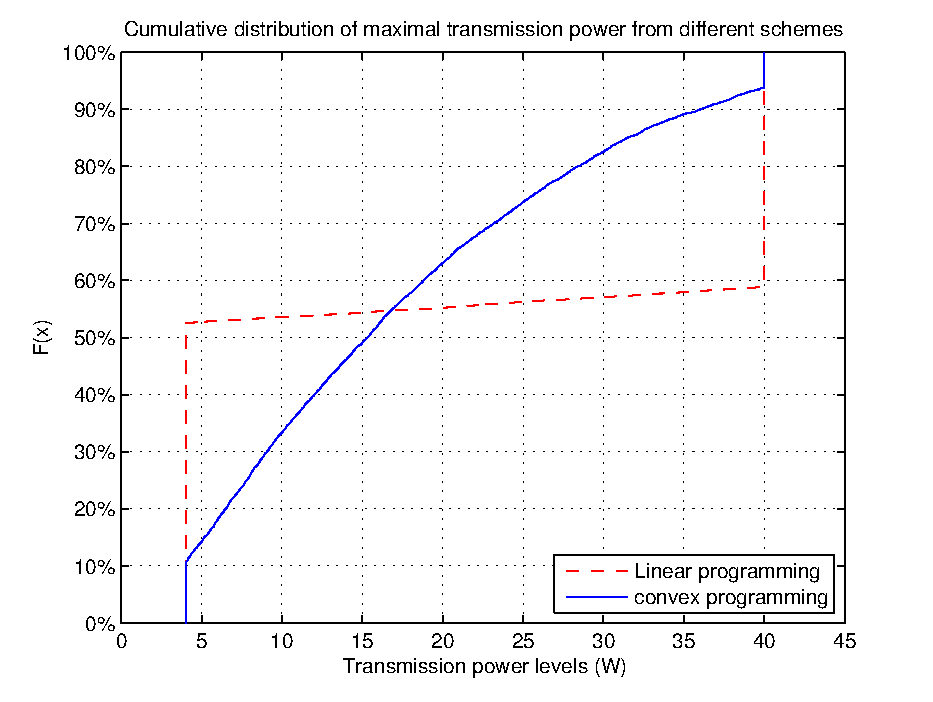
\includegraphics[width=0.89\linewidth]{lpcvxcdf100runs.pdf}
  \caption{Distribution of maximum permitted transmission power levels obtained from convex and linear programming formulations}
\label{lpcvx}
\end{figure}


Optimization problem \ref{cvx} provides the maximum permitted transmission power for each WBS and over each channel.
When all the WBSs working on the same channel, the generated interference doesn't exceed the threshold on the interference measurement devices at the contour of TV service area. 
If there are multiple channels available and WBSs are free to choose their preferred channels, the aggregate interference on one channel will be smaller than that when all WBSs work on that channel. 
Thus, there is exists a interference margin created by using multiple channels, which provides a room for network dynamics such as new WBS starting to work or increased interference on TV contour due to the variance of broadcast path condition. 
%XXX As mentioned above, it is not clear which impact the relationship between maximum transmit power planning and channel selection has XXX.


\section{Channel Allocation with Single Channel}
\label{CA_fixedPower_2subproblem}
%As discussed in~\ref{CA}, there is 
First, we give the centralized solution to obtain the global optimum for this subproblem, then the decentralized scheme under the game theoretic framework is introduced.

\subsection{Centralized Optimization Programming}
\label{03_centralized_ca}
We formulate the channel allocation problem into a binary quadratic programming problem which can be solved in a centralized way.  
Let $X_i = \{x_{i1}\cdots x_{ik}\cdots x_{i|\mathcal{C}|}\}$ denote the vector of channel usage, there is $|X_i| = |\mathcal{C}|$ and binary element $x_{ik}$ represent whether WBS $i$ occupies channel $k$.
For two WBSs $i$ and $j$, there is,
\begin{equation}
\begin{split}
X_i^TX_j = \sum\limits_{k=1}^{|\mathcal{C}|}x_{ik}\cdot x_{jk} = 
\left\{ \begin{array}{ll}
1 & \mbox{if $c_i=c_j$} \\
0 & \mbox{if $c_i\neq c_j$} 
\end{array}
\right.
\end{split}
\end{equation}

The power levels across all channels are denoted by a constant vector $P^{|\mathcal{C}|\times 1}$, which is possibly nonidentical to WBSs due to different locations. 
The power used by user $i$ is $P_i^TX_i = \sum\limits_{k=1}^{|\mathcal{C}|}P_{i}^k\cdot x_{ik}$.


Problem \ref{problem} can be modeled via general purpose nonlinear optimization:
	\begin{equation}
\label{QLP}
		\begin{aligned}
		& \underset{}{\text{minimize}}
		& & \sum\limits^{n}_{i=1} \frac{\sum\limits_{j\in\mathcal{N}, j\neq i}P^TX_j(X_j^TX_i)h_{ji}z_{ji} + N_0}{P^TX_ih_iz_i}\\
		& \text{subject to}
		& & \sum\limits_{k=1}^{|\mathcal{C}|}x_{ik}=1, x_{ik}\in X_i\in \{0,1\}^{|\mathcal{C}|}\\
		\end{aligned}
	\end{equation}
Problem \ref{QLP} is a non-linear problem with binary variables, but it can be reformulated in to a quadratic programming problem as,
	\begin{equation}
\label{QLP_2}
			\begin{aligned}
			& \underset{}{\text{minimize}}
			& &	\sum\limits^{n}_{i=1} ( \sum\limits_{j\in\mathcal{N}, j\neq i}\sum\limits_k \frac{P_{jk}\cdot h_{ji}\cdot z_{ji}}{P_{ik}\cdot h_i\cdot z_i}\cdot  x_{jk}\cdot x_{ik}  + \sum\limits_k \frac{N_0}{P_{ik}\cdot h_i\cdot z_i}\cdot x_{ik})\\
			& \text{subject to} 
			& & \sum\limits_{k=1}^{|\mathcal{C}|}x_{ik}=1, x_{ik}\in X_i\in \{0,1\}^{|\mathcal{C}|}\\
			\end{aligned}
		\end{equation}

The reformulation is available in Appendix \ref{optdeviation}.
We use LINDO~\cite{lindo} which is a state of art non-linear problem solver to solve the problem, which employs Branch-And-Reduce method to get the global optimum for the problem. % We use the results obtained by solving this QLP problem as one reference in the coming section. 
The result of this centralized channel assignment will be evaluated in the simulation section with other schemes. 



\subsection{Distributed White Space Channel Allocation (WitheCat): Algorithm and Protocol}
\label{whitecat}
In this section a distributed scheme for WBSs to allocate channels is proposed, which is named as \underline{white} space \underline{c}hannel \underline{a}llocation \underline{t}echnology (WitheCat). 
WitheCat adopts the best response process, where each WBS (referred as $i$) chooses the channel which brings the bigger utility $u_i$ as the response of other WBSs' choices on channels.
%and the sum of all WBSs' utilities is minimized after finite times of updates even the interaction between WBSs are asymmetric. The utility is as follows,
WitheCat is depicted by algorithm \ref{whitecatalgo}.

\begin{equation}
\label{utility}
u_i =\dfrac{\sum\limits_{\tiny\substack{j\in \mathcal{N}, j\ne i,\\ c(\sigma_j)=c(\sigma_i)}}f_{ji}}{2\cdot \tilde{P_i}} + \dfrac{1}{2}\sum_{\tiny\substack{j\in \mathcal{N}, j\ne i,\\ c(\sigma_j)=c(\sigma_i)}}\dfrac{f_{ij}}{\tilde{P_j}} + \sum_{\tiny\substack{\mathcal{S}:i,j\in \mathcal{S},\\ c(\sigma_j)=c(\sigma_i)}}\dfrac{N_0}{C\cdot \tilde{P_i}}\\
\end{equation}

where $f_{ij}= P_i\cdot h_{ij}\cdot z$ and $f_{ji}= P_j\cdot h_{ij}\cdot z$.
Note that $f_{ij}$ is the sum of interference on WBS $i$'s interference reference points.
Overlooking the constant coefficient 2, the first item of $u_i$ is a part of the inverted QuasiSINR of station $i$. 
To minimize the first item, WBS $i$ needs to choose a channel either permits higher transmission power or experiences less interference, whereas the higher power increases the second item which is a part of inverted QuasiSINR of other co-channel WBSs. 
Hence, the cost function presents a reasonable comprise between the welfare of one WBS and others.

When WBS only emphasizes on its own utility (e.g. the first part of Formula~\ref{utility}), the best response process doesn't converge.
We have following theorem:
\begin{theorem}
\label{noconvergence}
\emph{With non-identical transmission power, if every WBS updates its channel based on Algorithm \ref{whitecatalgo} with utility based on its own interests, the process doesn't always converge.}
\end{theorem}
The proof is in Appendix \ref{proof}.


\begin{algorithm}[h]
\caption{Spectrum selection by WBS $i$}          % give the algorithm a caption
\label{whitecatalgo} 
\DontPrintSemicolon
\SetAlgoLined
\KwIn{the distance, path lose and shadowing parameter between WBS $i$ to WBS $j\in \mathcal{N}\setminus i$;\\  radius of auxiliary circle, noise $N_0$, total number of WBSs $N$;\\ for $j\in \mathcal{N}\setminus i$, the maximal transmission power $P_j^c, c\in \mathcal{C}$ and the working channel $c(j)$.
}
%\KwOut{a channel }

	\For{$c\in \mathcal{C}\setminus c(i)$}{
	 calculate $u_i(c)$ based on Formula \ref{utility}
	 \eIf{$u_i(c)<u_i(c(i))$}{
	 	$c(i)\leftarrow c$
	 }
	 {keep $c(i)$ unchanged}
	}
	
Notify database of its channel usage, which further notifies the other WBSs

\end{algorithm}



%//废话
%Imitating the player's behaviour in the congestion game, each base station tries to find the channel $c\in \mathcal{C}$ that brings the smallest $u_i$ based on the other stations' decisions, every channel update decreases the summation of utilities in the whole network and finally converges to a pure Nash equilibrium (proof is in section \ref{game}.


Some parameters needed to calculate the utility are identical for all WBSs, such as quasi distance $e$, the total number of WBSs $N$, number of channels $C$, attenuation factor $\alpha$, standard deviation $\sigma_{WBS}$ in flat shadowing and noise $N_0$, albeit the following information is further needed to calculate $u_i$: 
	\begin{itemize} %{labelitemi}{$\bullet$}
	\item $\sum_{\tiny\substack{j\in \mathcal{N}, j\ne i,\\ c(\sigma_j)=c(\sigma_i)}}f_{ji}^c, c\in \mathcal{C}$: the received interference on $i$' virtual measurement point from other WBSs $j$ working on the same channel for $\forall c\in \mathcal{C}$.
	\item $ f_{ij}^c$: the interference caused by $i$ on $j$'s virtual measurement point when $i$ works on channel $\forall c\in \mathcal{C}$.
	\item $P_j^c$: transmission power of $j$ for using $\forall c\in \mathcal{C}$.
	\end{itemize}
Unfortunately, it is difficult to get these interferences of interested measured, for station $i$, it is low efficient to scan all channels and obtain the interferences $f_{ji}$ on virtual measurement point for each channel, furthermore, it is impossible to split the interference $f_{ij}$ from the total interference received on WBS $j$' virtual measurement point. 

We refer \cite{CApotentialLearning_05dyspan} to decide the sequence for WBSs to update their channel. \cite{CApotentialLearning_05dyspan} proposes a method like random access mechanism of CSMA/DA, where the access for broadcast medium is changed to getting access to the centralized center to retrieve the current channel usage and update its new channel. All WBSs are able to access the database in one round (with random or predetermined sequence). As WBSs are connected with database, the control messages needed to decide the sequence will not become a burden. Update of channels can happen in the boot phase, or when the quality of services (the SINR on its end users) of WBSs falls below a threshold, or a fixed time duration comes to end, or a new WBS joins in the network. 

Similar with~\cite{SenseLess2011}, we let every WBS store the location information and maximal power map of all other WBSs, \ie $P_i^c, i\in\mathcal{N}, c\in\mathcal{C}$, and each WBS retrieves information about channel usage of other WBSs from centralized base station.
After executing Algorithm \ref{whitecatalgo}, it reports to centralized database of its channel if it updates the working channel.
As the location of WBSs and TV stations and the transmission channel and power of TV stations are usually static (entries of TV station change averagely once in 2 days\cite{SenseLess2011}), except for the channel usage in the network, the change of the other data stored in WBS is infrequent. 


\subsection{Analysis in Game Theoretical Framework}
\label{game}
In this section, We give the proof on whiteCat's convergence in the framework of congestion game theory.
Formulating a spectrum sharing problem into a congestion game and the concept of \textit{virtual resources} are firstly proposed in \cite{allerton08_liu}.
This work reversely engineers the distributed channel allocation schemes proposed in \cite{babadi_08, Ko_DistributedCA}, \ie unifies the algorithms with congestion game.
But the problem analysed in~\cite{allerton08_liu} assume the transmission power is identical, which is a major difference from the channel allocation problem discussed here. 

%\subsubsection{Congestion Game}
%A congestion game \cite{Rosenthal}\cite{Voecking06congestiongames} can be expressed by a tuple $\lambda=(\mathcal{N},\mathcal{R},(\sum_i)_{i \in \mathcal{N}},(g_r)_{r\in \mathcal{R}})$, where $\mathcal{N}=\left\{1,\ldots,N\right\}$ denotes the set of players (each each is labeled with a unique index number), $\mathcal{R}=\left\{1,\ldots,m\right\}$ the set of resources, $\Sigma_{i\in\mathcal{N}} \subseteq 2^{\mathcal{R}}$ is the strategy space of player $i$. Under strategy profile $\sigma=(\sigma_1,\sigma_2,\cdots \sigma_N)$, player $i$ chooses strategy $\sigma_i\in \Sigma_i$, and the total number of users using resource $r$ is $n_r(\sigma)=|\{i\mid r\in \sigma_i\}|$. The cost $g_r: \mathbb{N}\rightarrow \mathbb{Z}$ is a function of the number of users for resource $r$, $g_r^i=\sum_{r\in \sigma_i} g_r(n_r(\sigma))$. In our paper, $g_r^i$ is referred as \textit{congestion} and is Monotonic.
%
%Rosenthal's potential function $\phi:\sigma_1\times\sigma_2\times\cdots\times\sigma_n\rightarrow Z$ is defined as:
%\begin{equation}
%\label{4}
%\begin{split}
%G(\sigma) 
%& =\sum\limits^{}_{r\in \mathcal{R}} \sum\limits^{n_r(\sigma)}_{i=1} g_r(i)\\
%& =\sum\limits_{i\in \mathcal{N}} \sum\limits^{}_{r\in \sigma_i} g_r(n_r^i(\sigma))\\
%\end{split}
%\end{equation}
%$n_r^i(\sigma)$ means the number of players using resource $r$ and \textit{their indices are smaller than or equal to $i$}. Note that the potential is \textit{not} the sum of congestions experienced by every user. The change of the potential caused by one player's unilateral move from $\sigma$ to $\sigma'$ is equivalent to the change of gain (or loss) of that player.
%\begin{equation}
%\label{5}
%\varDelta G(\sigma_i \rightarrow \sigma_i') = g^i(\sigma_i',\sigma_{-i}) - g^i(\sigma_i,\sigma_{-i})
%\end{equation}
%$\sigma_{-i}$ is the strategy profile for all players except for $i$.
%As every congestion game is a potential game, and the total potential is finite, thus the number of improvements is upper-bounded by $2\cdot\sum\limits^{}_{r\in \mathcal{R}} \sum\limits^{n_r(\sigma)}_{i=1} g_r(i)$ \cite{Voecking06congestiongames}.
%
%
We have introduced congestion game in Chapter~\ref{background}, thus we only recap the essence of congestion game here.
In congestion game, each player acts selfishly and aims at choosing strategy $\sigma_i\in \Sigma_i$ to minimize their individual cost.
The gain (loss) caused by any player's unilateral move is exactly the same as the gain (loss) in the potential, which may be viewed as a global objective function.
For problems where the potential of the problem is the same with the summation of the cost of all users, the cost function can be used as a utility function directly.
This equivalence doesn't exist in our problem, but by carefully choosing the cost function for players, we can make sure that the change of individuals' cost is in the same direction with that of the global utility.



\subsubsection*{The Congestion Game Formulated from the Algorithm WhiteCat}
\label{gameforproblem}
We utilize the conception of virtual resource which is firstly introduced in \cite{allerton08_liu}. 
Virtual resource is a triplet $\{i, j, c\}$, where $i,j$ are two WBSs and $c\in \mathcal{C}$ is one channel.
This piece of resource is regarded used by $i$ when both $i$ and $j$ use channel $c$, otherwise, $\{i, j, c\}$ is not used by any WBS.

In the following, we list the element of the congestion game which emulates Algorithm~\ref{whitecatalgo}.
In this section, player and base station are used interchangeably.

\begin{itemize}
\item Player $i$' strategy space is $\Sigma_i=\{(i,j,c), j\in \mathcal{N}, j\ne i, c(\sigma_j)=c, c=1,2,\cdots,N\}$, and $i$ has $C$ admissible strategies, one strategy related with channel $c\in\mathcal{C}$ is described by the set of virtual resources it uses: $\sigma_i=\{(i,j,c), j\in \mathcal{N}, j\ne i, c(\sigma_j)=c\}$, note that virtual resource $(i,j,c)\neq(j,i,c)$.

\item Under the strategy profile $\sigma=(\sigma_1, \sigma_2, \cdots \sigma_N)$, player $i$ obtains a total cost of 

	\begin{equation}
\label{6}
		\begin{split}
		g^i(\sigma)=
		& \sum\limits^{}_{\tiny\substack{j\in \mathcal{N},j\neq i,\\ c=c(\sigma_i)=c(\sigma_j)}} (g_{(i,j,c)}(n_{(i,j,c)}(\sigma))+g_{(j,i,c)}(n_{(j,i,c)}(\sigma))
		\end{split}
		\end{equation}
\end{itemize}

The transmission power over all channels of player $i$ is $\{p_i^1, p_i^2,\cdots, p_i^{|\mathcal{C}|}\}$.
%According to our system model, interfere xxxxxx
%Path loss is assumed reciprocal: $h_{ij}=h_{ji}$, but nor is the flat fading $z$. To keep the formula clear in the following part, we denote $\tilde{f_{ij}}= P_i\cdot h_{ij}\cdot z$, $\tilde{f_{ji}}= P_j\cdot h_{ij}\cdot z$, $\tilde{P_i}=h_{iQ}$ for $i\in \mathcal{N}$, where $h_{ji}=h_{ij}=(d_{ji}-e)^{-\alpha}, h_{ii}=h_{jj}=e^{-\alpha}$, $d_{ji}$ is the distance between base station $i$ and $j$, and $\delta$ is the quasi distance introduced in section \ref{SystemModel}. $N_0$ is noise which is identical for any channel and any WBS. 
We define the cost function for virtual recourses $(i,j,c)$ as follows,
\begin{equation}
\label{costfuc4resrc}
\begin{split}
g_{(i,j,c)}(k) = 
\left\{ \begin{array}{ll}
%\tilde{f_{ji}}/(2\tilde{P_i}) + f_{ij}/(2\tilde{P_j}) + N_0/(C\cdot \tilde{P_i})\\\\
%=\dfrac{P_j\cdot h_{ji}\cdot z/2 + N_0/C}{P_i\cdot h_{iQ}\cdot z} +\dfrac{P_i\cdot h_{ij}\cdot z/2}{P_j\cdot h_{jQ}\cdot z} & \mbox{if $k=2$} \\
\dfrac{f_{ji}}{2\tilde{P_i}} + \dfrac{f_{ij}}{2\tilde{P_j}} + \dfrac{C\cdot N_0}{N\cdot \tilde{P_i}} & \mbox{if $k=2$} \\
%=\dfrac{P_j\cdot h_{ji}\cdot z/2 + N_0/C}{P_i\cdot h_{iQ}\cdot z} +\dfrac{P_i\cdot h_{ij}\cdot z/2}{P_j\cdot h_{jQ}\cdot z} & \mbox{if $k=2$} \\
0 & \mbox{otherwise}
\end{array}
\right.
\end{split}
\end{equation}


As resource $(i,j,c)$ only lies in the strategy space of player $i$ and $j$, thus can only be accessed by this two players.
More specifically, according to Formula~\ref{costfuc4resrc}, the cost of resource $(i,j,c)$ is only decided by the number of players using it, which is either 0 or 2.
At the first glance, this is a player specific congestion game, as $g_{(i,j,c)}$ is decided by the relevant players' transmission power and inference.
But actually the resource ${(i,j,c)}$ excludes the players except for $i$ and $j$ from using it, thus the cost happened on this resource is only dependant on how many of players from the set $\{i, j\}$ to use it.
Hence, the cost is a function of the number of players using the resource, and this is a canonical congestion game.

\subsubsection*{Bridging the Game and Algorithm WhiteCat}

When we substitute Formula \ref{costfuc4resrc} to Formula \ref{6}, the total cost for user $i$ under strategy profile $\sigma$ . 

\begin{equation}
\label{cost1player}
\begin{split}
g^i(\sigma)
%& = \sum_{\tiny\substack{j\in \mathcal{N}\setminus i,\\ c=c(\sigma_j)=c(\sigma_i)}} g_{(i,j,c)}(2) + \sum_{\tiny\substack{j\in \mathcal{N}, j\ne i,\\ c=c(\sigma_j)=c(\sigma_i)}} g_{(j,i,c)}(2)\\
& = \sum_{\tiny\substack{j\in \mathcal{N}\setminus i,\\ c=c(\sigma_j)=c(\sigma_i)}} (g_{(i,j,c)}(2) + g_{(j,i,c)}(2))\\
%& = \sum_{\tiny\substack{j\in \mathcal{N}, j\ne i,\\ c(\sigma_j)=c(\sigma_i)}} (\dfrac{f_{ji}/2 + N_0/C}{\tilde{P_i}} + \dfrac{f_{ij}/2}{\tilde{P_j}})\\
& = \sum_{\tiny\substack{j\in \mathcal{N}\setminus i,\\ c(\sigma_j)=c(\sigma_i)}}(\dfrac{f_{ji}}{\tilde{P_i}} + \dfrac{f_{ij}}{\tilde{P_j}}+ \dfrac{C\cdot N_0}{N}(\dfrac{1}{\tilde P_i}+\dfrac{1}{\tilde P_j})) \\
& = \dfrac{\sum\limits_{\tiny\substack{j\in \mathcal{N}\setminus i,\\ c(\sigma_j)=c(\sigma_i)}}f_{ji}}{ \tilde{P_i}} + \sum_{\tiny\substack{j\in \mathcal{N}\setminus i, \\c(\sigma_j)=c(\sigma_i)}}\dfrac{f_{ij}}{\tilde{P_j}} + \dfrac{CN_0}{N}\sum_{\tiny\substack{j\in \mathcal{N}\setminus i,\\ c(\sigma_j)=c(\sigma_i)}}(\dfrac{1}{\tilde{P_i}}+\dfrac{1}{\tilde{P_j}})\\
& = \dfrac{\sum\limits_{\tiny\substack{j\in \mathcal{N}\setminus i,\\ c(\sigma_j)=c(\sigma_i)}}f_{ji}}{ \tilde{P_i}} + \sum_{\tiny\substack{j\in \mathcal{N}\setminus i,\\ c(\sigma_j)=c(\sigma_i)}}\dfrac{f_{ij}}{\tilde{P_j}} + \dfrac{2CN_0}{N}\sum_{\tiny\substack{i\in\mathcal{S}\subset\mathcal{N},\\\mathcal{S}:\forall i\in \mathcal{S}\\ c(\sigma_i)=c}}\dfrac{1}{\tilde{P_i}}\\
\end{split}
\end{equation}

where $\mathcal{S}$ denotes the set of WBSs whose working channel is the same with WBS $i$.

Now we are going to have a look at the \textit{potential} of the network.
According to the expression of Rosenthal's potential in Formula~\ref{2:Rosenthal_potential_newdelay}, the potential is accumulated by adding the players' cost sequentially, in particular, the value which is added is the cost that player experiences when it starts to use the relevant resource, and the value is not changed when other players come to use that resource.
Back to our problem, for two WBSs $i,j\in \mathcal{S}$, we assume WBS $i$'s index is smaller than $j$'s index, then the potential increased by $i$ using the resource $\{i,j,c\}$ is 0 according to Formula~\ref{6}, and the increase brought in by $j$ using the resource $\{i,j,c\}$ is $g_{(i,j,c)}(2)+g_{(j,i,c)}(2)$. 
In other words, for each interfering pair of WBSs, only the WBS with bigger index contributes to the potential. 
Then the total potential is, 
\begin{equation}
\label{allPotential}
\begin{split}	
G(\sigma) 
& =\sum\limits^{}_{r\in \mathcal{R}} \sum\limits^{n_r(\sigma)}_{i=1} g_r(i)  =\sum\limits_{i\in \mathcal{N}} \sum\limits^{}_{r\in \sigma_i} g_r(n_r^i(\sigma))\\
%& = \sum\limits_{i\in \mathcal{N}}\dfrac{\sum\limits_{\tiny\substack{j\in \mathcal{N}, j\ne i,\\ c(\sigma_j)=c(\sigma_i)}}\tilde{f_{ji}}}{\tilde{P_i}} + \sum\limits_{\tiny\substack{\mathcal{S}\backepsilon i, \mathcal{S}\subset \mathcal{N},\\ \forall j\in \mathcal{S}, j\neq i,\\ c(\sigma_j)=c(\sigma_i)}}  (\dfrac{\mid\mathcal{S}\setminus 1 \mid}{C} \frac{N_0}{\tilde{P_i}})
& = \sum\limits_{i\in \mathcal{N}}\dfrac{\sum\limits_{\tiny\substack{j\in \mathcal{N}, j\ne i,\\ c(\sigma_j)=c(\sigma_i)}}f_{ji}}{\tilde{P_i}} + \dfrac{CN_0}{N}\sum\limits_{\tiny\substack{\mathcal{S}\subset \mathcal{N},\\ \forall i\in \mathcal{S}, c(\sigma_i)=c}} \mid \mathcal{S}\mid   \sum\limits_{\tiny\substack{i\in \mathcal{S}}}\frac{1}{\tilde{P_i}}
\end{split}
\end{equation}

 note that the summation of one WBS's congestion is related to its index. 

%Question:
%
%When power is variable, is it still a congestion game, or potential game?

When players minimize their utilities (cost or potential) illustrated by Formula \ref{cost1player}, the total congestion in the secondary network given by Formula \ref{allPotential} decreases monotonically before reaching one Nash equilibrium. Players' greedy update in the game to minimize its cost Function\ref{cost1player}, which ceases finally in pure Nash Equilibrium. The strategy and cost function of players in the game is transplanted as Algorithm \ref{whitecatalgo} and utility Function \ref{utility} respectively.


\subsubsection*{Gap between the Potential of Game and the Objective}
It is natural to raise the question, is the sum of the final utilities of all WBSs exactly the same with the value of potential when the game converges to a Nash equilibrium, which is represented by \ref{allPotential}?
The answer is, they are identical when $N_0$ is zero, and there will be a little difference when $N_0$ is not zero.
Recall the target objective we want to minimize in Problem \ref{problem} is,
\begin{equation}
\label{compare}
\begin{split}	
\sum_{i\in \mathcal{N}}\dfrac{f_i}{\tilde{P_i}}
& = \sum\limits_{i\in \mathcal{N}}\dfrac{\sum_{\tiny\substack{j\in \mathcal{N}, j\ne i,\\ c(\sigma_j)=c(\sigma_i)}}f_{ji}+N_0}{\tilde{P_i}}\\
& = \sum\limits_{i\in \mathcal{N}}\dfrac{\sum_{\tiny\substack{j\in \mathcal{N}, j\ne i,\\ c(\sigma_j)=c(\sigma_i)}}f_{ji}}{\tilde{P_i}} + \sum\limits_{i\in \mathcal{N}}  (\dfrac{N_0}{\tilde{P_i}})\\
\end{split}
\end{equation}
We notice that only the last items of the objective~\ref{compare} and the potential of the congestion game~\ref{allPotential} are different.
When $N_0=0$, the potential is exactly the same with the object we want to minimize.
When $N_0\neq 0$, if channels are evenly distributed and there is $C/N*\mid \mathcal{S}\mid = 1$, then Formula~\ref{compare} and \ref{allPotential} are also the same.
In both cases, the sum of utilities \ref{compare} decreases monotonically with every update of WBSs before the system reaches Nash Equilibrium.
%
When $N_0\neq 0$ and Formula~\ref{compare} and \ref{allPotential} are thus different, the monotonicity on the decrease of sum of utilities \ref{compare} is not perceived, whereas the system will still cease to NE.

Based on above analysis, we can see the assumption that each WBS only occupies one channel can be easily removed.
If we regard one WBS as multiple ones which locate at the same place, and each WBS works on one distinct channel, then the proof on convergence of whiteCat can be applied directly to this case.

Note that the convergence of the game is independent on the the concrete form of the cost function. 
We adopt the function \ref{cost1player} to let the potential of the game be the same with the total utility of all WBSs, so that by executing Algorithm~\ref{whitecatalgo}, the system objective experiences a monotonic decreasing process before the system reaching NE.
The algorithm has potential to solve many other problems, where one user's decision affects others.
In this case, the utility of one user can be formulated to incorporate the information of its own utility and others', then the congestion game theory can be used to analogize.
%Hence, WhiteCat scheme provides a prototype for the problems where the interaction among users are asymmetric.



\subsubsection*{Communication Overhead of WhiteCat}

The problem of channel allocation with different and fixed transmission power is NP hard.
WhiteCat is a distributed scheme but certain information of the other WBSs is needed.
The centralized base station is piggybacked to provided the needed information.
As to one WBS, the number of such inquiries is the number of steps before convergence.

In our formulated congestion game, a player $i$ is allowed to access up to $(N-1)$ resources in the same time, \ie $\{i, j_1, c(i)\}, \{i, j_2, c(i)\} \cdots \{i, j_{N-1}, c(i)\}$, thus the upper bound of converge steps can not be obtained from the conclusion~\ref{2:Rosenthal_potential_newdelay} for singleton congestion game.
But our problem is special because for each resource, the possible number of players allowed to use each resource is either 2 or 0.
Thus we can refer the method used in Section~\ref{singleton_congestion_game} to analyse the update times for our problem.
Firstly, we sort the cost values in increasing order.
Although a WBS 
\begin{equation}
\label{2:Rosenthal_potential_newdelay}
\begin{split}
\phi(\sigma) 
& =\sum\limits^{}_{r\in \mathcal{R}} \sum\limits^{n_r(\sigma)}_{i=1} g_r(i)\\
& \leq \sum\limits^{}_{r\in \mathcal{R}} \sum\limits^{n_r(\sigma)}_{i=1} n\\
& \leq n^2m
\end{split}
\end{equation}

The upper bound of total update steps is $2n^2$, thus averagely, the upper bound of update steps for each WBS is $2n$.



\section{Channel Allocation with Multiple Channels}
Both of the proposed centralized and distributed channel allocation schemes, which are initially designed for single channel allocation, can be easily adapted to solve the multiple TV channel allocation problem which complies with ECC rulings.

As to the distributed scheme allocating multiple channels for WBSs, we regard a WBS working on a certain channel as a \textit{logic} WBS, in other words, a WBSs operating on multiple channels can be seen as multiple co-location logic WBSs and each of them operates on a single channel respectively. 
The logic WBSs work complying with the algorithm~\ref{whitecatalgo}, and the convergence also applies in this process.

As to the centralized solution, the constraint in the optimization formulation~\ref{QLP_2} needs to be changed as,

	\begin{equation*}
		\sum\limits_{k=1}^{|\mathcal{C}|}x_{ik}=w, x_{ik}\in X_i\in \{0,1\}^{|\mathcal{C}|}\\
	\end{equation*}
where $w$ is the number of channels for each WBS to operate.

\section{Performance Evaluation}
\label{simulation}
Performance evaluation consists with three parts.
In the first part we investigate the choice of radius of the auxiliary circle.
Then the comparison between our proposed schemes which work with single channel and the other distributed schemes are conducted.
In this process, the channel-power maps which are obtained from linear and convex optimization are used respectively.
In the last part, we compare the proposed schemes working with different amount of channels with a distributed scheme which is designed complying with FCC rulings.



The evaluation setting is as follows and some parameters are listed in Table~\ref{6}.
A square area which is 60km x 60km is divided evenly into 16 square blocks.
There is one WBS sitting in the middle of each block,  where its end terminals are distributed within the same block.
There is a 20km wide rim area around the square area, where the critical points for the DTV receivers are randomly located.
The locations of WBSs and TV contours are illustrated in Fig.~\ref{sim:layout}.
WBSs' locations are fixed, but the end terminals, and the sequence for WBS to update are randomly decided in each run.
In each run the critical points for the digital TV service are located at different places, so that the power-channel map for every WBS is different in different runs.
Each simulation was repeated 50 times and the mean along with its 95 percent confidence interval is plotted for every measurement. 

\begin{figure}[h!]
  \centering
  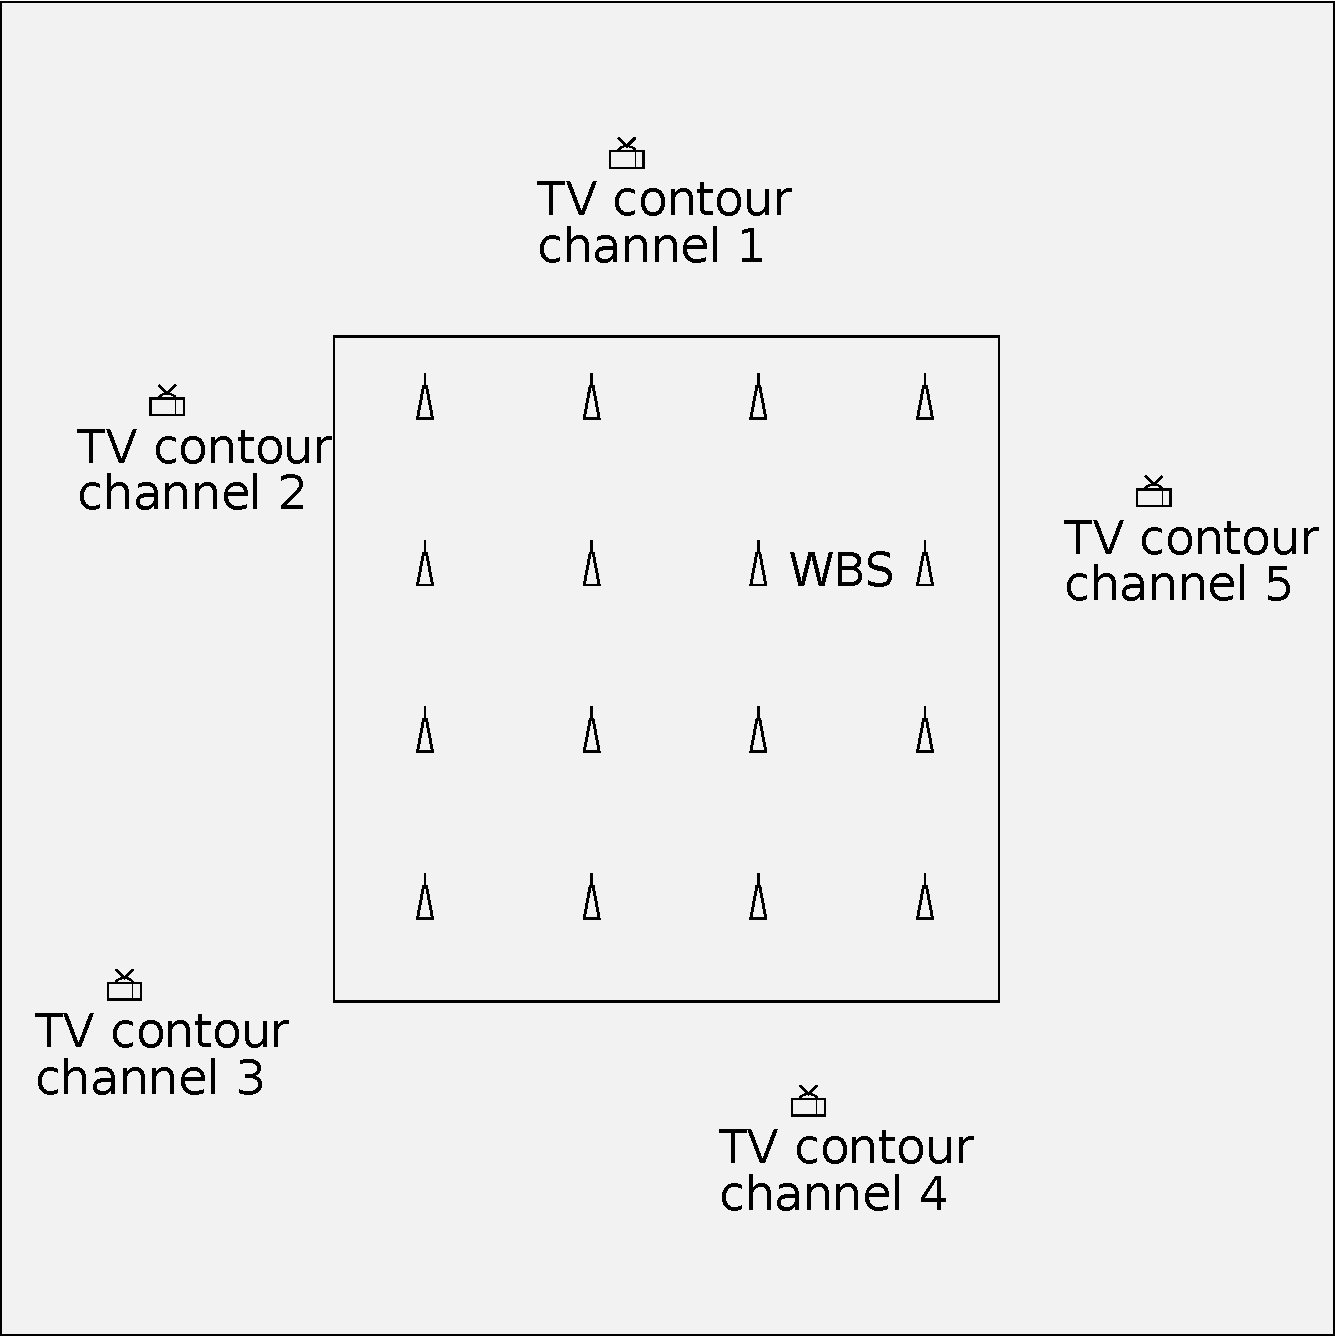
\includegraphics[width=0.5\linewidth]{layout.pdf}
  \caption{Layout of WBSs and TV contours}
  \label{sim:layout}
\end{figure}

The other parameters are listed in Table~\ref{6}.

\begin{table}[!h]
\centering
\begin{tabular}{|l|r|}
  \hline
  Number of channels 						& 4 \\
  Number of WBSs							& 9, 16\\
  Noise 									& $10^{-13}$ Watt \\ % -90dbm
  Side length of area hosting WBSs		& 60 km\\
  Auxiliary circle radius 	& 1 km \\
  Inf. threshold on critical point 		& $10^{-8}$, 5x$10^{-8}$ Watt \\ % -67dbm
  Path loss factor 							& 2 \\
  Standard deviation in flat shadowing		& 8\\
  Number of end terminals per cell 		& 10 \\
  Min. WBS Tx power 			& 1 Watt \\
  Max. WBS Tx power			& 4 Watt \\
  Number of simulation runs & 50 \\

  \hline
\end{tabular}
\caption{Simulation parameters}
\label{simulationparameter}
\end{table}


\subsection{The Choice of Radius of Auxiliary Circles, quasiSINR of WBS, and SINR on End Users}
The usage of quasiSINR exempts WBSs from taking care the SINR on the end terminals.
A WBS's quasiSINR is related with WBS's location and the radius of auxiliary circle.
Figure~\ref{radius} illustrates the effect of using different radii of the auxiliary circle on the data rate can be achieved by end terminals.

\begin{figure}[h]
\centering
\subfigure[quasiSINR of WBSs]{
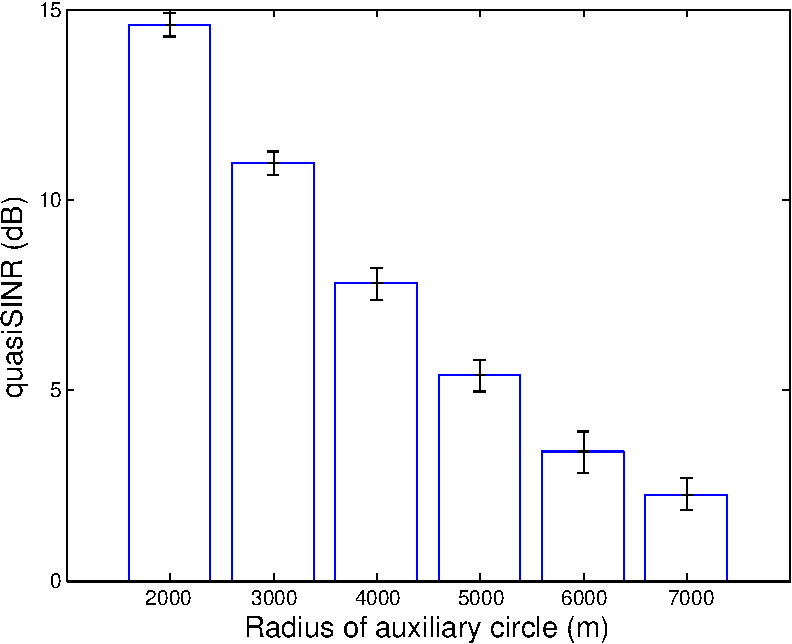
\includegraphics[width=0.435\linewidth]{qusaiSINR_with_radius.pdf}
\label{qusaiSINR_with_radius}
}
\subfigure[Data rate of end terminals when applying whiteCat]{
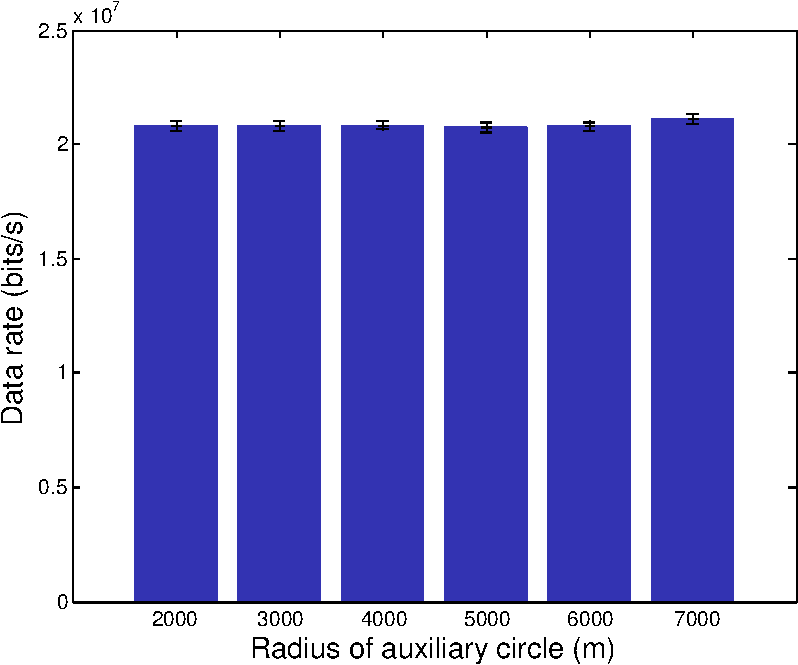
\includegraphics[width=0.435\linewidth]{sinr_on_endusers_with_radius.pdf}
\label{sinr_on_endusers_with_radius}
}
\caption[]{The effects of different radii of auxiliary circle on end terminals' data rate. Maximum permitted power is obtained by solving convex optimization. WhiteCat is used to assign the channels.}
\label{radius}
\end{figure}

Subfigure~\ref{qusaiSINR_with_radius} shows WBSs' quasiSINR decreases when the radii of auxiliary circles increase.
Subfigure~\ref{sinr_on_endusers_with_radius} illustrates the choice on radius of auxiliary circle don't influence the performance of whiteCat.
In the following simulation, we fixed the radius at 6000 m.

     


\subsection{Performance of Channel Allocation Schemes Operating with Single Channel}
\label{single_channel_performance}
The comparison schemes are \textit{whiteCase} and No-regret learning, besides, centralized optimization is used to obtain global optima.
\begin{itemize}
\item \textit{WhiteCase}:  \underline{White}space \underline{c}hannel \underline{a}llocation \underline{se}lfish, where each WBS selfishly updates its channel to achieve the best (as to the considered problem, smallest) possible utility based on Formula~\ref{selfishutility}.
\item \textit{Noregret learning}: Each WBS maps the probability of choosing each strategy to a certain proportion of the regret which the WBS may have if it doesn't choose that strategy, and the WBS choose the strategy with the biggest probability.  
WBSs update such mapping dynamically and this approach converges to correlated equilibrium. 
Please refer the original paper \cite{hart00correlatedeq} for details.
\item \textit{Quadratic optimization}: centralized quadratic optimization introduced in Section~\ref{03_centralized_ca}.
\end{itemize}

In Section~\ref{powermap}, two different optimization formulations are introduced to obtain the channel-power map for WBSs, \ie convex optimization and linear optimization respectively.
In Figure~\ref{lpcvx}, we have seen the convex optimization generates power levels which distribute evenly between the minimum and maximum transmission power levels configured by the hardware, while, the majority of the power levels generated by linear optimization are either the minimum or maximum transmission power.
The simulation in this subsection carries twofold meanings.
The first is to see which channel-power map outperforms the other, the second is to evaluate the performance of the channel allocation schemes.
The adopted metrics are the SINR on end terminals and transmission power consumption.


\subsubsection{Comparison of the Methods for Maximum Permitted Transmission Power}
%We simulate the 4 distributed spectrum allocation schemes with the  map obtained from , and then tell which maximal power map generation outperforms based on the performances of the 4 spectrum allocation schemes.
 
Figure~\ref{transPower} depicts the power consumption of the channel allocation schemes which work with the two groups of maximum permitted transmission power decided by linear and convex problems respectively.
When given maximum permitted transmission power, whiteCat and the centralized optimization scheme consume the least energy.
The schemes utilize less transmission power with the maximum permitted transmission power decided by convex optimization.
%
Figure~\ref{qusaiSINR} shows the quasiSINR of WBSs.
The centralized optimization scheme achieves the highest quasiSINR, because the optimization formulation~\ref{QLP} obtains the global optima.
 \begin{figure}[h!]
    \centering
      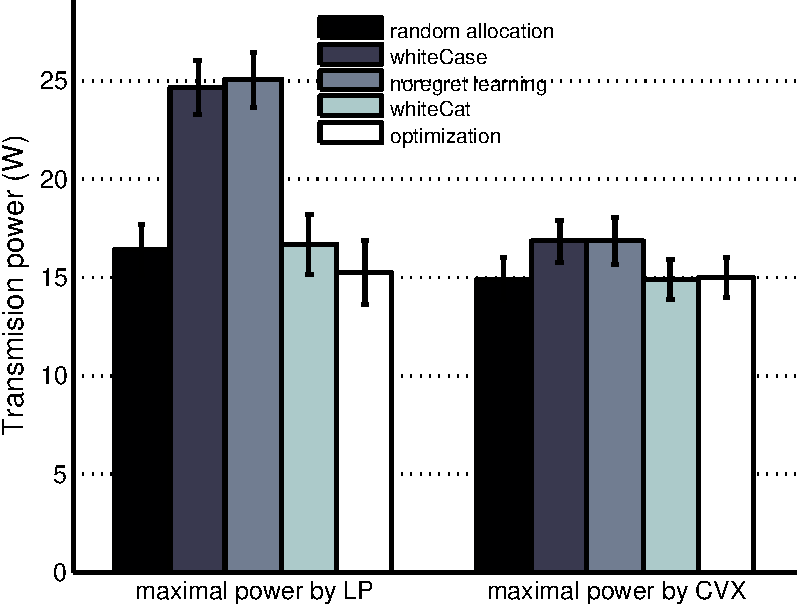
\includegraphics[width=0.7\linewidth]{transPower.pdf}
    \caption{Power consumed of WBSs by different distributed spectrum allocation schemes under different ways deciding the maximal transmission power map}
\label{transPower}    
  \end{figure}
  
   \begin{figure}[h!]
       \centering
       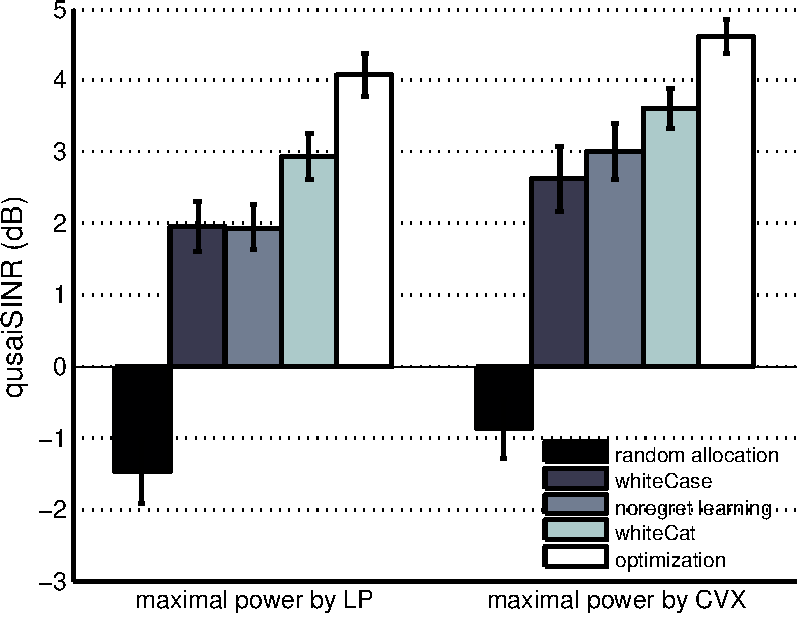
\includegraphics[width=0.7\linewidth]{qusaiSINR.pdf}
       \caption{QuasiSINR of WBSs achieved by different distributed spectrum allocation schemes under different ways deciding the maximal transmission power map}
	\label{qusaiSINR}
     \end{figure}
     
The average SINR on the end terminals is depicted in Figure~\ref{6000_sinr}.
When the given maximum permitted transmission power, whiteCat and the centralized optimization achieve similar and the best performance among the schemes.
It is also noticed that, the maximum permitted transmission power decided by linear optimization helps the channel allocation schemes achieve better SINR.
     \begin{figure}[h!]
       \centering
       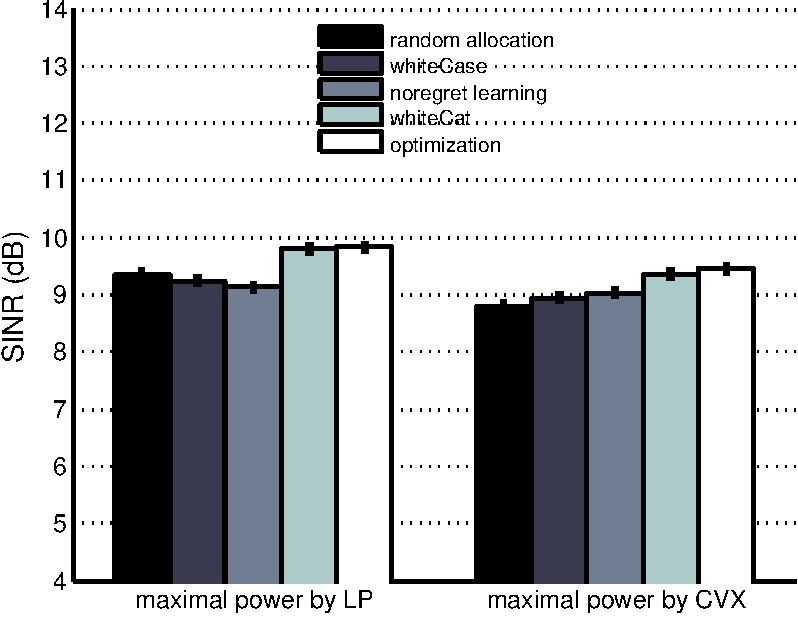
\includegraphics[width=0.7\linewidth]{6000_sinr.pdf}
       \caption{SINR on end terminals achieved by different distributed spectrum allocation schemes under different ways deciding the maximal transmission power map}
	\label{6000_sinr}
     \end{figure}

  \begin{figure}[h!]
     \centering
     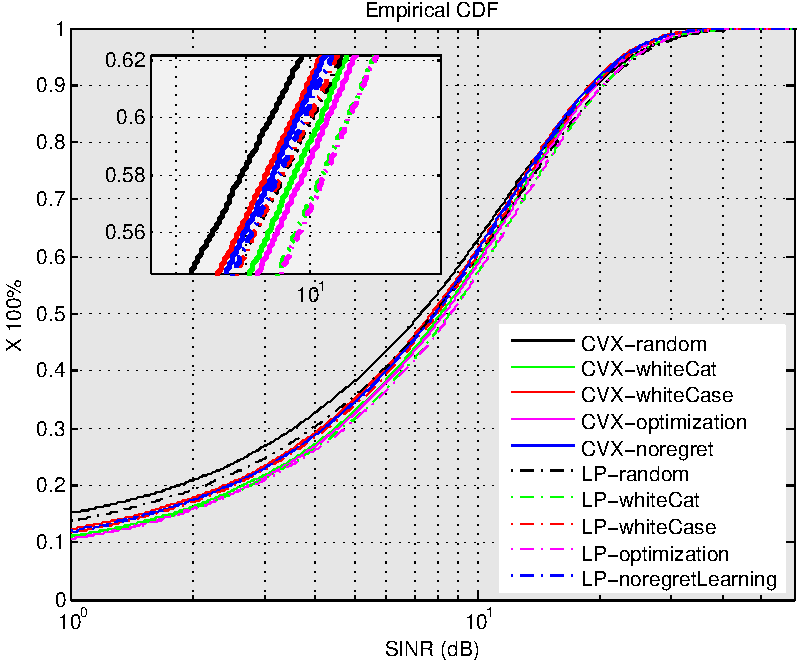
\includegraphics[width=0.7\linewidth]{6000_sinr_cdf.pdf}
     \caption{CDF of SINR on end users obtained by different CA schemes under different methods to decide the maximal transmission power map}
     \label{6000_sinr_cdf}
  \end{figure}

The empirical cumulative distribution function curve of SINR on end terminals is drawn in Figure \ref{6000_sinr_cdf}.

The SINR achieved by WhiteCat and the centralized optimization is stably higher than that obtained from other schemes.
For example, the 20\% and 80\% percentile of the SINR achieved by WhiteCat and the centralized optimization are 0.5 to 1 dB higher than the other channel allocation schemes.


\subsubsection{Convergence Speed}

%Complexity: 
%For each player, there are at most $(n-1)*|\mathcal{C}|$ resources available for usage, while, because the produced congestion on each resource is independent on channel, in other words, the congestions involving the same pair of players are quantitatively identical, there are only $(n-1)$ quantitatively different congestions on one player's resources. So, the number of combinations with quantitatively non-identical congestions involved with that player is $2^{(n-1)}$, accordingly there are totally $n*2^{(n-1)}$ quantitatively different congestions for the whole the problem. We adopt the method of \cite{LectureA}, which resorts the congestions in a increasing sequence, and replaces the original congestions with integer values starting form 1. We call the integers as \textit{new} congestions. In this way the preferences of the players are preserved and we can find easily the biggest possible congestion is $n*2^{(n-1)}$, which is the upper bound for the number of steps towards convergence.
In the congestion game where scheme whiteCat is derived, each player (WBS) has at most $(n-1)*|\mathcal{C}|$ resources available for usage, thus there is no polynomial steps converging to NE, while, simulation shows the algorithm can quickly converge to NE when the number of WBS is up to 100. 
%Figure \ref{100converge} shows that for 100 WBSs, whitecat executes at most 5 iterations (in one iteration all WBSs update their choices). 
%Figure \ref{convergeComp} depicts one instance of simulation, where whiteCat converges quickly, No-regret produces oscillation but converges finally, while WhiteCase can not converge thus has to be enforced stop after 16000 updates. %\todo{replot}%, whereas 
%
Table~\ref{convergencespeed} shows the average number of steps needed before convergence in 100 runs of simulations.
As to whiteCat, we account each WBS accessing the base station (refer to \ref{whitecat}) as \textit{one step}.
We compare the convergence speed of WhteCat with no-regret learning, the scheme derived from potential game~\cite{pimrc_2012} and whiteCase.
Note that the potential game scheme is to solve joint power and channel allocation problem, as it is developed with game theory, it is reasonable to see its convergence speed.
As there is no guarantee for WhiteCase to converge, we stop the channel allocation process after 16000 steps (1000 rounds).

Table~\ref{convergencespeed} tells that whiteCat is two times faster than the scheme derived from potential game, and 20 times faster than no-regret learning scheme.
The relatively smaller confidence interval shows that whiteCat's convergence is not affected by different network configurations.
Fast converge is attributed to the working style of WBSs whcih access the database to get the information of other WBSs, thus the distributable decision involves a part of the global information of the network.
Thus, we can see that the speed up of convergence is due to the overhead caused by accessing the database.


Figure \ref{convergeComp} depicts one instance of the convergence processes of three schemes.
The Y axis is the summed utility of all WBSs.
We can see whiteCat decreases the summed utility constantly, and the channel allocation process ceases after 38 times of updates.
Whereas, noregret learning scheme takes 120 steps before convergence, and whiteCase fails to converge.
%XXXXXX ***************
%Notice that there is a slight rise when the value on the X-axis is 35, which comes from the difference between \ref{compare} and \ref{allPotential}.
%XXXXXX ***************
\begin{table}[!h]
\centering
\begin{tabular}{|l|c|c|c|}
  \hline
  Scheme			 						& Average steps 	 		& 95\% CI			&Average time (s)\\
    \hhline{|=|=|=|=|}
  whiteCat									& 58						& 5.6						&2\\\hline
  noregret									& 1916						& 1541						&144\\\hline
  PotentialGame~\cite{pimrc_2012}			& 120						& 10						&4\\\hline
  optimization-LINDO						& -                         & -                         &40\\\hline
  whiteCase 								& 4587 						& 2742						&50\\  
  \hline
\end{tabular}
\caption{Convergence speed of the distributed channel allocation schemes. As to the distributed scheme, the time involved to communicate with database is note considered and included.}
\label{convergencespeed}
\end{table}

%\begin{figure}[h!]
%\label{100converge}
%  \centering
%  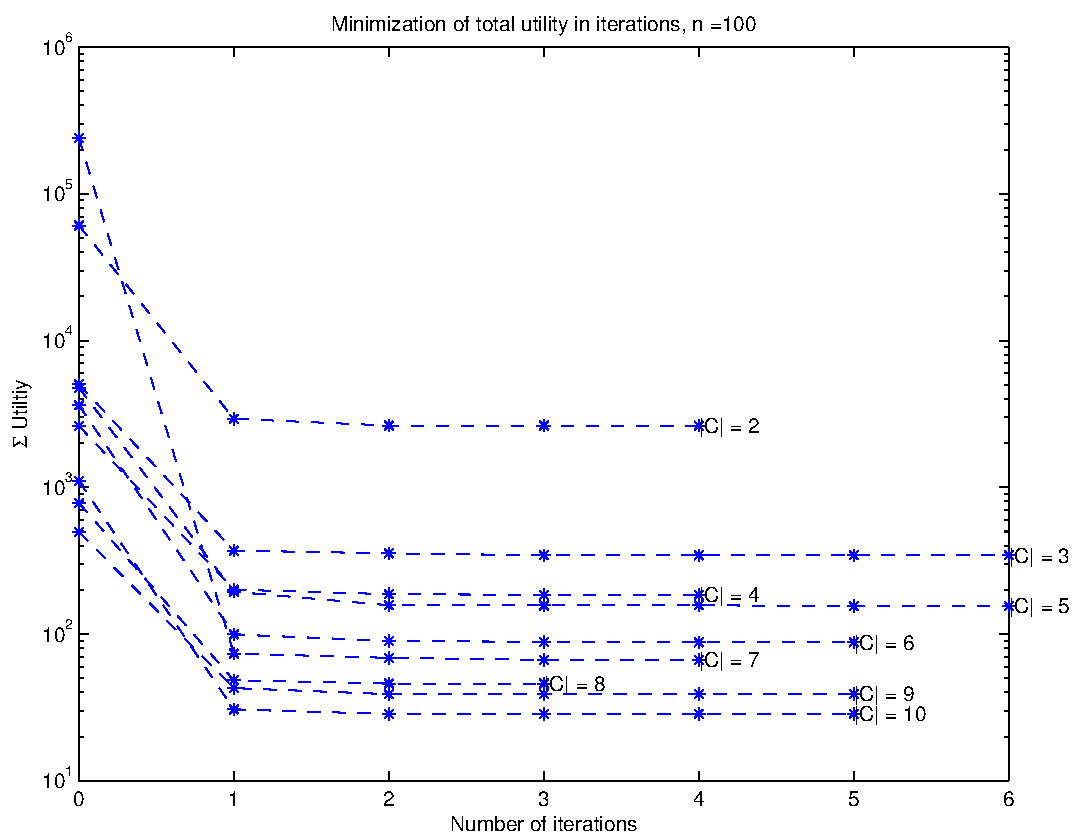
\includegraphics[width=0.65\linewidth]{CAConverenge100.pdf}
%  \caption{100 WBSs, 2-10 channels}
%\end{figure}

\begin{figure}[h!]
  \centering
  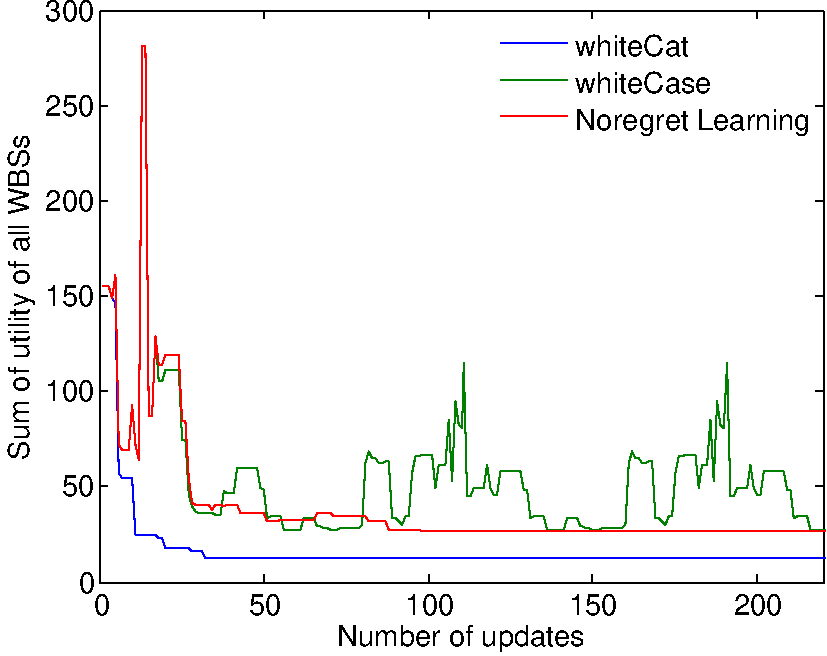
\includegraphics[width=0.8\linewidth]{convergence.pdf}
  \caption{Convergence process of three different schemes in one simulation.}
\label{convergeComp}
\end{figure}




%\subsubsection*{Stability of SINR in Convergence Process}
%WBS provides service to end users in the process of channel allocation. 
%A certain SINR corresponds to certain transmission configurations like modulation type and data rate. 
%The oscillation of SINR resulted from WBS changing the working channel during the convergence process may cause reconfiguration, reduced throughput or delay variance, which is not preferred.
%We propose a metric \textit{Cost of Oscillation} (\gls{COS}) to represent the stability of SINR in the converging process.
%Assuming each update of channel takes 1 time unit, the variance of SINR of end user $i$ at time $t+1$ is \[\varDelta  \gamma_i(t+1)=\mid\frac{\gamma_i(t+1)-\gamma_i(t)}{\gamma_i(t)} \mid\]. 
%
%The COS value for one network applied with a certain channel allocation scheme is,
%\begin{equation}
%\label{cos}
%			COS = \sum\limits_{t=1}^T   \sum\limits_{i\in \mathcal{N}} \varDelta  \gamma_i(t)
%			\end{equation}
%$\gamma_i(0)$ is the SINR for $i$ before starting channel allocation.
%The variance of SINR in channel allocation process is shown in table \ref{costable} from which we can see WhiteCat achieves only 6\% of oscillation on SINR compared with No-regret approach.
%\begin{table}[!h]
%\centering
%\begin{tabular}{|l|c|c|}
%  \hline
%  Scheme			 						& COS 					& 95\% confidence interval\\
%    \hhline{|=|=|=|}
%  WhiteCat									& 8850					& 2984\\\hline
%  No-regret									& 145460				& 1541\\\hline
%  WhiteCase 								& 246790 				& 168050\\ 
%  \hline
%\end{tabular}
%\caption{Variance of SINR during the convergence process}
%\label{costable}
%\end{table}
%

\subsection{Performance of Channel Allocation Schemes Operating with Single Channel}
\label{Multiple_channel_performance}
As comparison, we implement the centralized scheme proposed in~\cite{ReAlloTVWS14DySPAN} (code can be found at~\cite{GreedyAlo}), which is designed complying with FCC regulations.
Some adaptions are made to comply with the ECC rulings, 1) When a channel is chosen, the WBS transmits with the maximal permitted transmission power permitted on that channel instead of an identical power for all the WBSs; 2) Auxiliary circle is introduced into the scheme, and the SINR is not the quotient of the transmission power and the interference on the WBSs' locations, but the power of signal and interference on the auxiliary circles.


The first group of simulation is conducted with 9 WBSs which locate as a 3 X 3 array, there are 4 TVWS channels.
Figure~\ref{transPower} and~\ref{ECC_multiChannel_Capacity} depict the average transmission power of all the WBSs and average capacity over all the end user when working with different amount of channels.
Figure~\ref{transPower_each_cell} and~\ref{ECC_multiChannel_Capacity_each_cell} illustrate the average transmission power and capacity for each WBS over all simulation runs. 
The two proposed schemes have similar performances which increase linearly with the number of TVWS channels in use.
The greedy scheme consumes as less power as our proposed schemes when single channel is used, because many WBSs are in idle state by adopting the greedy scheme.
The average Shannon capacity is also comparable to our proposed schemes.
When more channels are allowed, our proposed schemes clearly outperform the greedy scheme in terms of achieved Shannon capacity, with the cost of high transmission power.

 \begin{figure}[h!]
    \centering
      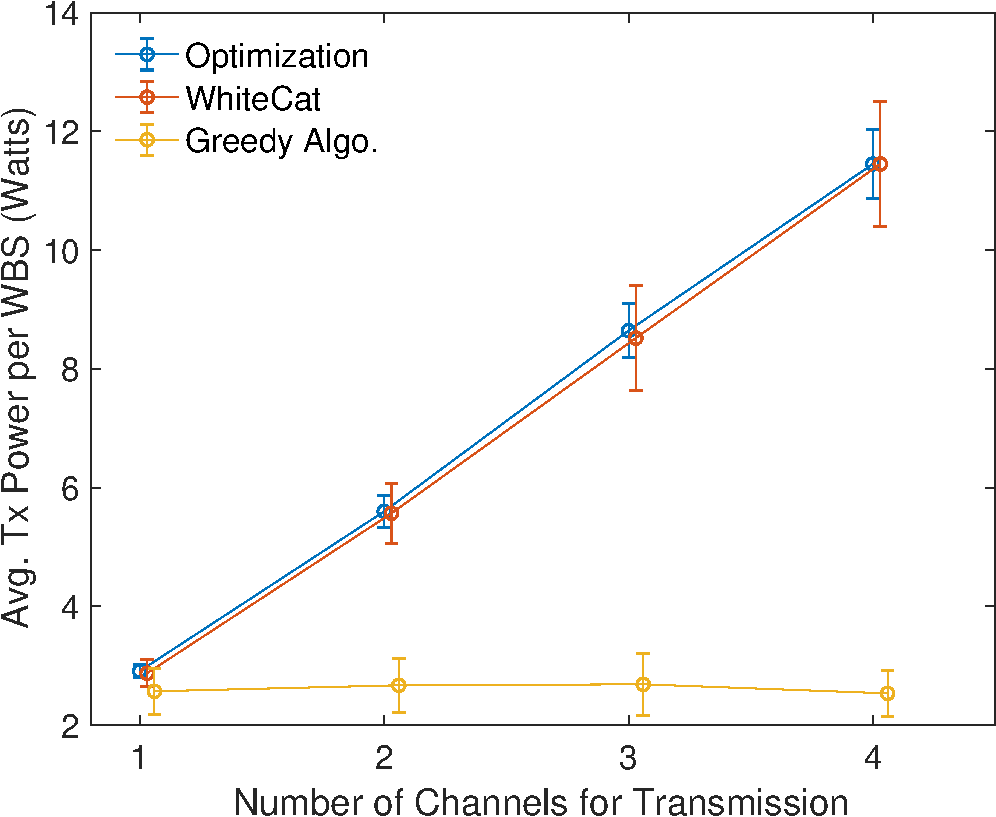
\includegraphics[width=0.8\linewidth]{ECC_multiChannel_withComparison_Tx_1000_9WBS-crop.pdf}
    \caption{Average transmission power of all WBSs, 9 WBSs, 4 channels.}
\label{transPower}    
  \end{figure}
  
     \begin{figure}[h!]
       \centering
       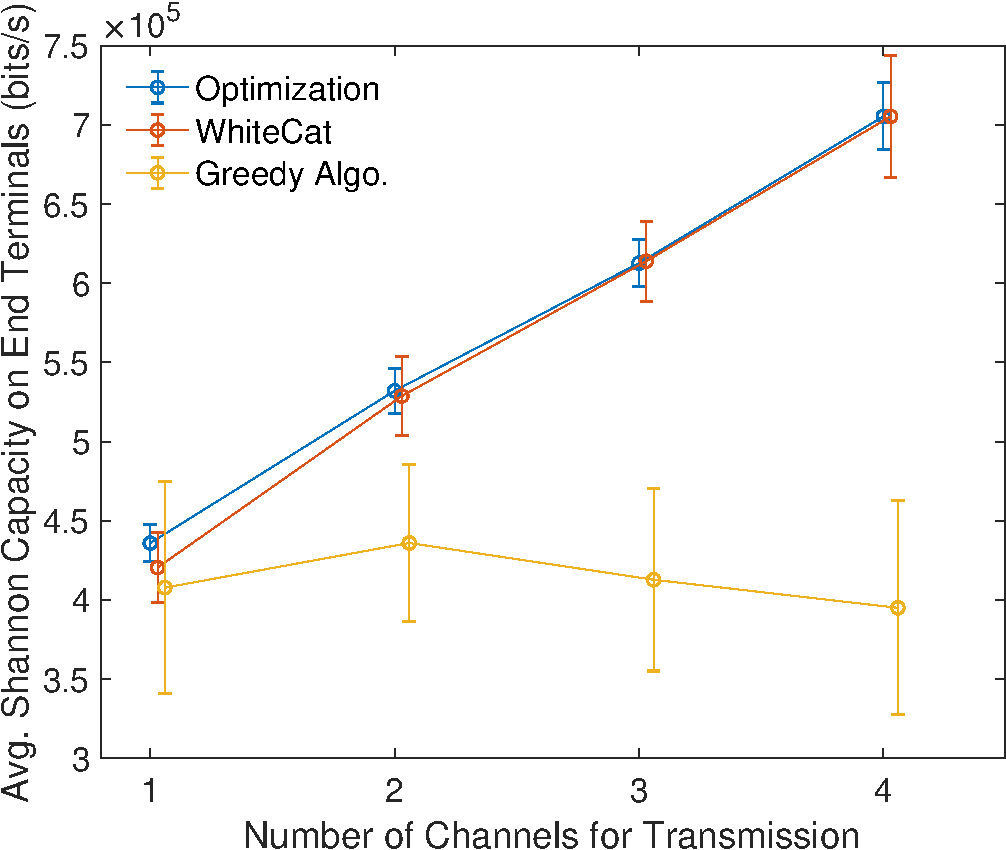
\includegraphics[width=0.8\linewidth]{ECC_multiChannel_withComparison_Capacity_1000_9WBS-crop.pdf}
       \caption{Average capacity over all end terminals,  9 WBSs, 4 channels.}
	\label{ECC_multiChannel_Capacity}
     \end{figure}
%------------------------------------
 \begin{figure}[h!]
    \centering
      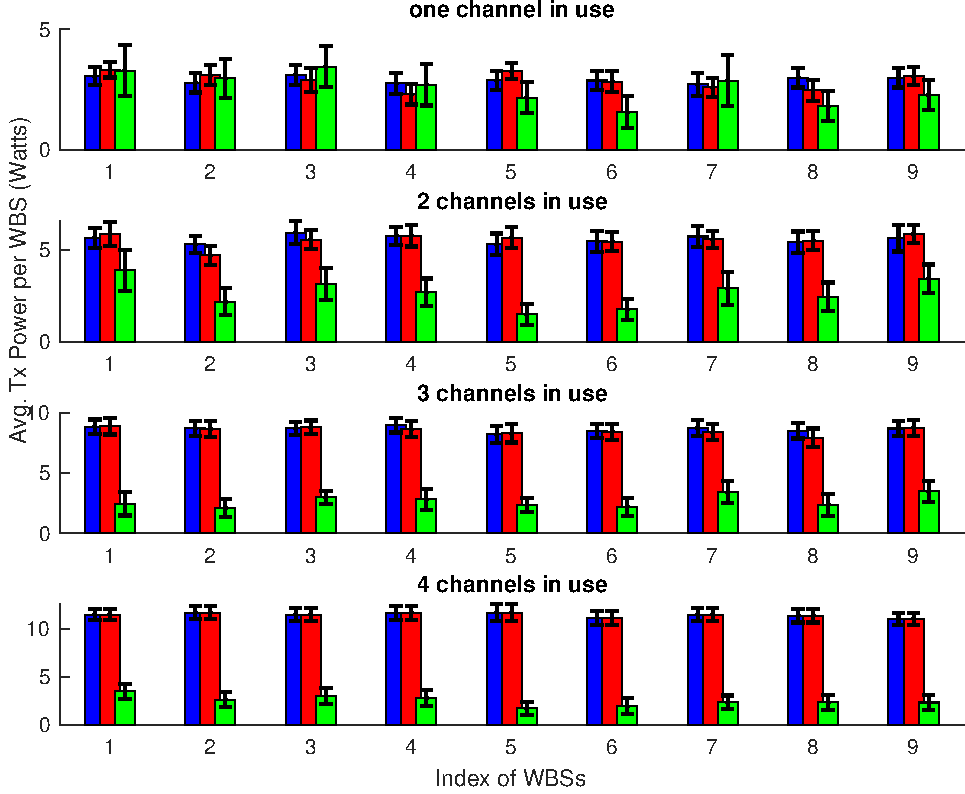
\includegraphics[width=0.8\linewidth]{ECC_multiChannel_withComparison_Tx_All_9_WBS-crop.pdf}
    \caption{Average transmission power of each WBS, 9 WBSs, 4 available channels. Increasing number of channels (1 to 4 channels) are used from top to bottom.}
\label{transPower_each_cell}    
  \end{figure}
  
     \begin{figure}[h!]
       \centering
       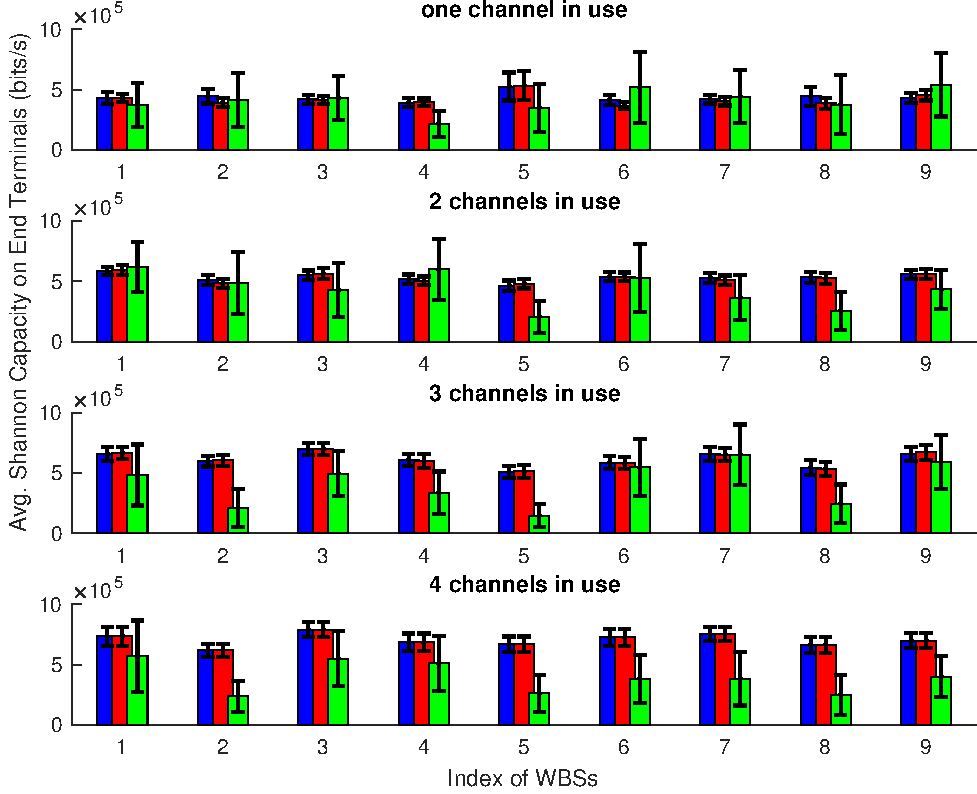
\includegraphics[width=0.8\linewidth]{ECC_multiChannel_withComparison_Capacity_All_9_WBS-crop.pdf}
       \caption{Average capacity of end terminals in each WBS's cell,  9 WBSs, 4 available channels. Increasing number of channels (1 to 4 channels) are used from top to bottom.}
	\label{ECC_multiChannel_Capacity_each_cell}
     \end{figure}


The second group of simulation is done with 16 WBSs, which is a denser scenario than group 1. 
The average transmission power of WBSs and average capacity on end users, as shown in~\ref{transPower2} and~\ref{ECC_multiChannel_Capacity2}, are similar when implying the proposed centralized and distributed schemes.
Figure~\ref{transPower2_each_cell} and Figure~\ref{ECC_multiChannel_Capacity2_each_cell} depict the average transmission power and Shannon capacity in each WBS cell.
Comparing with group 1, less transmission power is consumed by all the three investigated schemes, and meanwhile the achieved capacity is less.
This is because the network is denser in group 2 and the co-channel interference has bigger impact on the WBSs.
The greedy scheme is liable to generate more idle WBSs, as a result, both of the transmission power and Shannon capacity are less than our proposed schemes.


 \begin{figure}[h!]
    \centering
      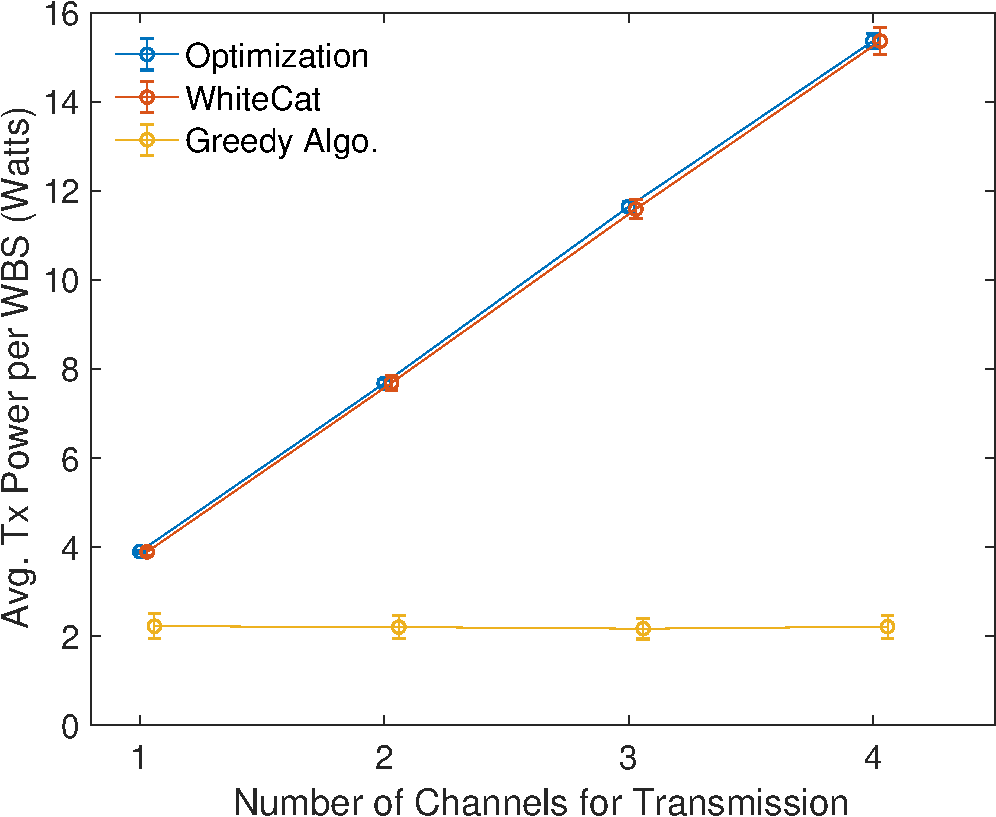
\includegraphics[width=0.8\linewidth]{ECC_multiChannel_withComparison_Tx_1000_16WBS-crop.pdf}
    \caption{Average transmission power of WBSs,  16 WBSs, 4 channels.}
\label{transPower2}    
  \end{figure}
  
       \begin{figure}[h!]
       \centering
       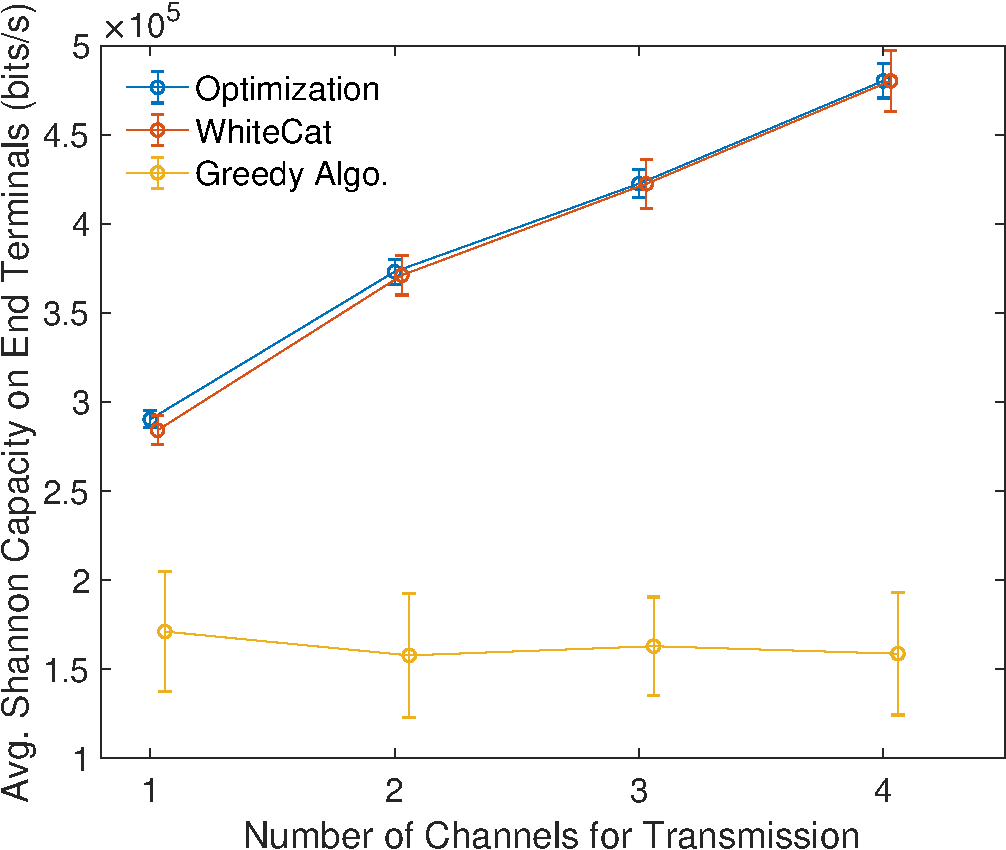
\includegraphics[width=0.8\linewidth]{ECC_multiChannel_withComparison_Capacity_1000_16WBS-crop.pdf}
       \caption{Average capacity on end terminals,  16 WBSs, 4 channels.}
	\label{ECC_multiChannel_Capacity2}
     \end{figure}
%-----
 \begin{figure}[h!]
    \centering
      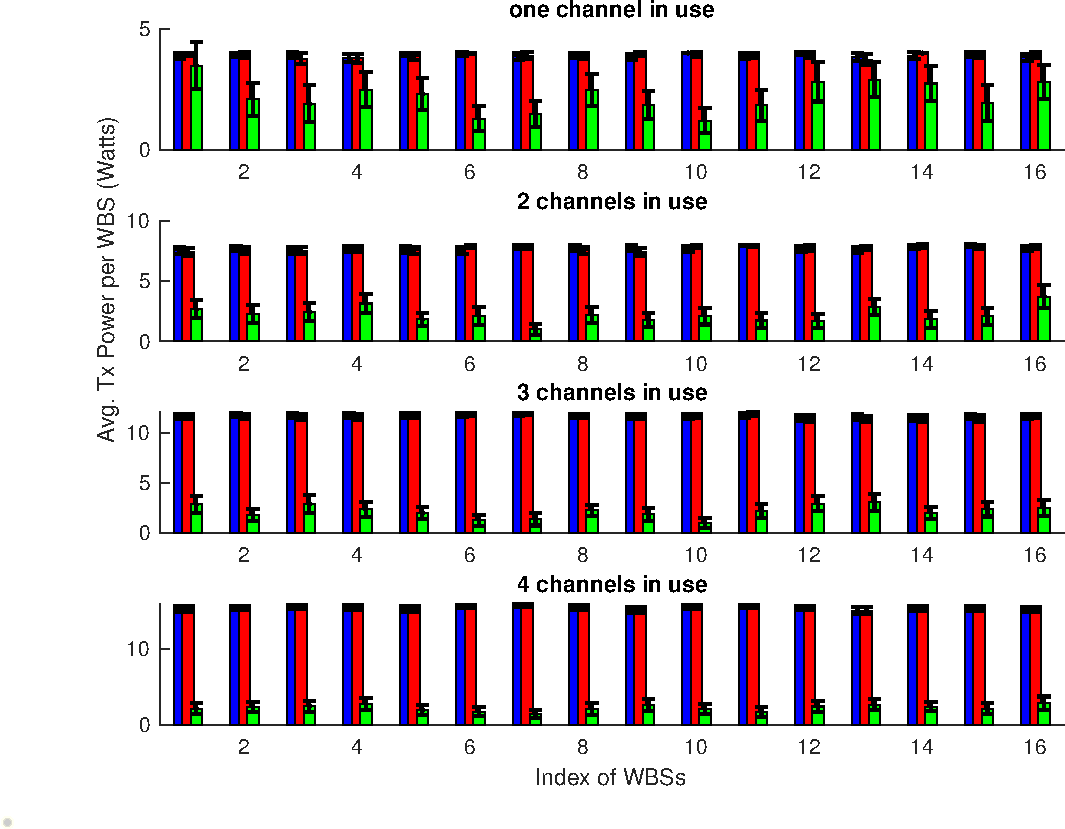
\includegraphics[width=0.81\linewidth]{ECC_multiChannel_withComparison_Tx_All_16_WBS-crop.pdf}
    \caption{Average transmission power of WBSs,  16 WBSs, 4 available channels. Increasing number of channels (1 to 4 channels) are used from top to bottom.}
\label{transPower2_each_cell}    
  \end{figure}
  
       \begin{figure}[h!]
       \centering
       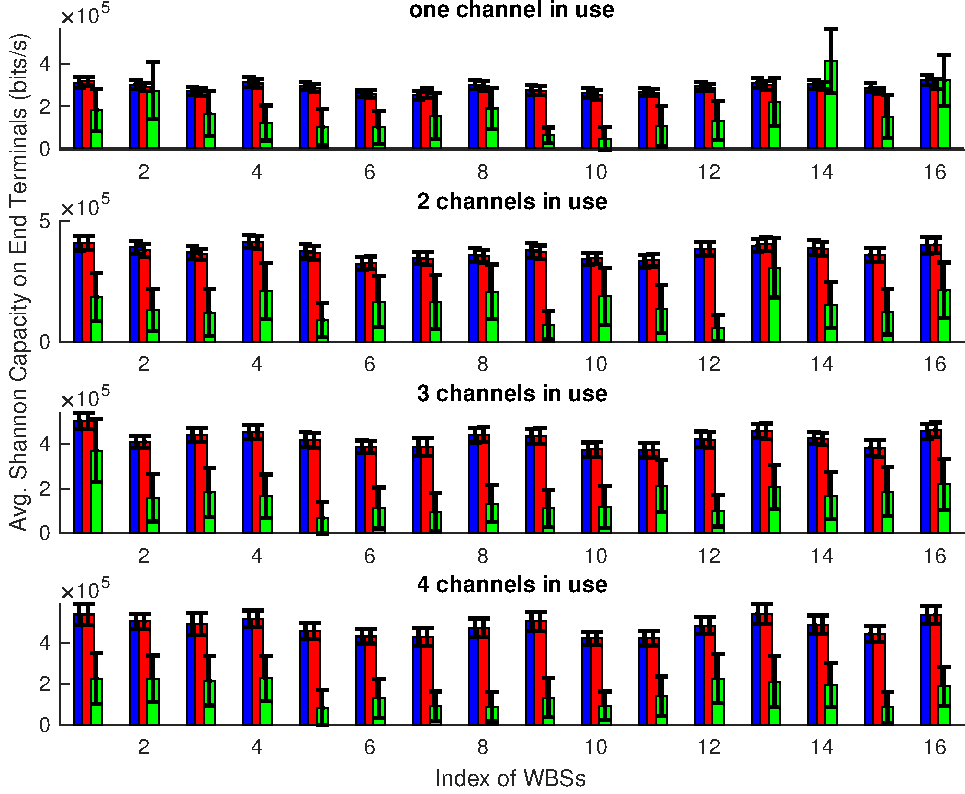
\includegraphics[width=0.8\linewidth]{ECC_multiChannel_withComparison_Capacity_All_16_WBS-crop.pdf}
       \caption{Average capacity on end terminals,  16 WBSs, 4 available channels. Increasing number of channels (1 to 4 channels) are used from top to bottom.}
	\label{ECC_multiChannel_Capacity2_each_cell}
     \end{figure}

\section{Conclusions}
Congestion game is applied to analyse the channel allocation problem, where transmission power is not necessarily identical.
The proposed algorithm which is derived from the best response of the congestion game converges quickly, and achieves better performance than other distributed schemes.
Without consider the communication latency between WBSs and the database, this distributed scheme executes much faster than the centralized scheme.

In particular, we investigate the channel allocation problem in the context of utilization of TV white space.
Except for channel allocation, we also propose solutions for transmission power control for the cellular network which complies with IEEE 802.22 standard.
%With the centralized database, a centralized method to obtain the maximum permitted transmission power which complies with IEEE 802.22 standard is proposed.
%Then a distributed channel allocation algorithm is designed based on congestion game, where WBS can distributively choose the working channel which is associated with maximum permitted transmission power.
%The distributed channel allocation scheme outperforms several other distributed solutions, and obtains worse performance only than the centralized solution, while.

%A transmission power control procedure is conducted on the previous channel allocation.
%We investigate the performance of applying the combination of channel allocation and the power control.
%Our proposed channel allocation scheme together with power control achieve better performance than the other channel allocation scheme with the same power control scheme.
%The centralized joint channel and power scheme performs the best, but the problem is very difficult to solve.

%This solution makes full use of the infrastructure, the centralized database, and distributes the computation and decision making afterwards on channel and transmission power.




